 %% Copyright (C) 2011, Andrea Cimino, All Rights Reserved.
 %% This file is distributed under the terms of the Creative Commons
 %% Licence Non-Commercial Share-Alike license

%%26 Ottobre
%% Useful stuff for separate compilation.
\ifx\ismaindoc\undefined
\providecommand{\inbpdocument}{
 \documentclass[11pt,a4paper,twoside,titlepage]{scrbook}
%%%%%%%%%%%%%%%%%%%%%%%%%%%%%%%%
%%%%%%%%%%% PACKAGES %%%%%%%%%%%
%%%%%%%%%%%%%%%%%%%%%%%%%%%%%%%%
% encoding
\usepackage[utf8x]{inputenc}
\usepackage[italian]{babel} % babel (suddivisione parole in sillabe)

\usepackage{amsfonts} % matematica
\usepackage{amsmath} % matematica
\usepackage{amssymb} % simboli vari
\usepackage{calrsfs}
\usepackage{caption}
\usepackage{enumerate}
\usepackage{extarrows} % matematica
\usepackage{keyval}
\usepackage{manfnt} % Simboli curva
\usepackage{mathtools} % matematica
\usepackage{multirow} 
\usepackage[usenames, dvipsnames]{color} % colori con nome
\usepackage[pdftex]{graphicx}
\usepackage{epstopdf} % gestione file EPS
\usepackage{wrapfig} % per figure circondate da testo
\usepackage{framed}	% teoremi framed
\usepackage{fancyhdr} % header buffi
\usepackage[T1]{fontenc} % gestione hbox e vbox
\usepackage[a4paper]{geometry}
\usepackage{microtype} % gestione hbox e vbox
\usepackage[thref, amsthm, amsmath, framed, hyperref]{ntheorem} % teoremi (avanzata)
%% \usepackage{prooftree} % gestione prof-tree
\usepackage{rotating}
\usepackage{stmaryrd}
\usepackage{subfig}
\usepackage{syntax} % syntattic stuff
\usepackage{txfonts}
\usepackage{verbatim} % migliorie al verbatim
%\usepackage{hyperref}
%% \usepackage{qtree}
\usepackage{fancyvrb}
\usepackage{listings}
\usepackage{cancel}
\usepackage{tikz}

\usepackage{bbding} %% Icons

%%%%%%%%%%%%%%%%%%%%%%%%%%%%%%%%
%%%%%%%%%%% GEOMETRY %%%%%%%%%%%
%%%%%%%%%%%%%%%%%%%%%%%%%%%%%%%%
\geometry{verbose,tmargin=2cm,bmargin=2.5cm,lmargin=2.5cm,rmargin=2cm}
\parindent0ex %% Remove paragraph indenting

%%%%%%%%%%%%%%%%%%%%%%%%%%%%%%%%
%%%%%%%%%%% CODE ENV %%%%%%%%%%%
%%%%%%%%%%%%%%%%%%%%%%%%%%%%%%%%
% codice
\newcounter{count}
\setcounter{count}{0}
\newenvironment{code}[1]
{
\color{lightgray}\hrulefill\color{code}
\stepcounter{count} {\bf\small Listato di codice \arabic{count}: {#1} }
\verbatim
}
{
\endverbatim
\color{lightgray}\hrulefill
\color{black}
\\
}

% codice semplice
\newenvironment{simplecode}
{
\color{code} \tt
}
{
\rm
}

 % Notation issues

%% Proof trees.
%\input prooftree
\newcommand*{\nohyp}{\phantom{x}}

%% C++.
\newcommand*{\Cplusplus}{{C\nolinebreak[4]\hspace{-.05em}\raisebox{.4ex}
{\tiny\bf ++}}}

%% BNF rules.
\newcommand*{\vbar}{\mathrel{\mid}}

%% Abstract syntax of the analyzed language.
\newcommand*{\Type}{\mathrm{Type}}
\newcommand*{\dType}{\mathrm{dType}}
\newcommand*{\dT}{\mathrm{dT}}
\newcommand*{\sType}{\mathrm{sType}}
\newcommand*{\sT}{\mathrm{sT}}
\newcommand*{\cType}{\mathrm{cType}}
\newcommand*{\cT}{\mathrm{cT}}
\newcommand*{\Integer}{\mathrm{Integer}}
\newcommand*{\Bool}{\mathrm{Bool}}
\newcommand*{\Id}{\mathrm{Id}}
\newcommand*{\id}{\mathrm{id}}
\newcommand*{\rId}{\mathrm{rId}}
\newcommand*{\idx}{\mathrm{x}}
\newcommand*{\ridx}{\underline{\mathrm{x}}}
\newcommand*{\Exp}{\mathrm{Exp}}
\newcommand*{\Exps}{\mathrm{Exps}}
\newcommand*{\Decl}{\mathrm{Decl}}
\newcommand*{\exceptDecl}{\mathrm{exceptDecl}}
\newcommand*{\Catch}{\mathrm{Catch}}
\newcommand*{\Stmt}{\mathrm{Stmt}}
\newcommand*{\Label}{\mathrm{Label}}
\newcommand*{\Con}{\mathrm{Con}}
\newcommand*{\con}{\mathrm{con}}
\newcommand*{\fps}{\mathrm{fps}}
\newcommand*{\funBody}{\mathrm{Body}}
\newcommand*{\funbody}{\mathrm{body}}
\newcommand*{\main}{\mathrm{main}}
\newcommand*{\es}{\mathrm{es}}
\newcommand*{\formParams}{\mathrm{formParams}}
\newcommand*{\emptysequence}{\boxempty}
\newcommand*{\Glob}{\mathrm{Glob}}

%% Sets of configurations
\newcommand*{\NTe}{\Gamma_\mathrm{e}}
\newcommand*{\NTb}{\Gamma_\mathrm{b}}
\newcommand*{\NTd}{\Gamma_\mathrm{d}}
\newcommand*{\NTg}{\Gamma_\mathrm{g}}
\newcommand*{\NTs}{\Gamma_\mathrm{s}}
\newcommand*{\NTk}{\Gamma_\mathrm{k}}
\newcommand*{\Te}{T_\mathrm{e}}
\newcommand*{\Tb}{T_\mathrm{b}}
\newcommand*{\Td}{T_\mathrm{d}}
\newcommand*{\Tg}{T_\mathrm{g}}
\newcommand*{\Ts}{T_\mathrm{s}}
\newcommand*{\Tk}{T_\mathrm{k}}

%% Lambda notation.
\newcommand*{\lambdaop}{\mathop{\lambda}\nolimits}

%% Sets of (no better specified) configurations.
\newcommand*{\NT}[1]{\Gamma_{#1}}
\newcommand*{\NTq}{\Gamma_q}
\newcommand*{\Tq}{T_q}

%% Denotable values.
\newcommand*{\dVal}{\mathrm{dVal}}
%% Storeable values.
\newcommand*{\sVal}{\mathrm{sVal}}
\newcommand*{\sval}{\mathrm{sval}}

%% Control modes.
\newcommand*{\CtrlMode}{\mathord{\mathrm{CtrlMode}}}
\newcommand*{\cm}{\mathrm{cm}}
%% Branch modes.
%\newcommand*{\BranchMode}{\mathord{\mathrm{BranchMode}}}
\newcommand*{\GotoMode}{\mathord{\mathrm{GotoMode}}}
\newcommand*{\SwitchMode}{\mathord{\mathrm{SwitchMode}}}
\newcommand*{\cmgoto}{\mathop{\mathrm{goto}}\nolimits}
\newcommand*{\cmswitch}{\mathop{\mathrm{switch}}\nolimits}
\newcommand*{\cmbreak}{\mathop{\mathrm{break}}\nolimits}
\newcommand*{\cmcontinue}{\mathop{\mathrm{continue}}\nolimits}
\newcommand*{\cmreturn}{\mathop{\mathrm{return}}\nolimits}
%% Exec mode.
\newcommand*{\cmexec}{\mathrm{exec}}
%% Value mode.
\newcommand*{\ValMode}{\mathord{\mathrm{ValMode}}}
\newcommand*{\cmvalue}{\mathop{\mathrm{value}}\nolimits}
%% Environment mode.
\newcommand*{\EnvMode}{\mathord{\mathrm{EnvMode}}}
\newcommand*{\cmenv}{\mathrm{env}}
%% Exception modes.
\newcommand*{\ExceptMode}{\mathord{\mathrm{ExceptMode}}}
\newcommand*{\cmexcept}{\mathrm{except}}

%% Control states.
\newcommand*{\CtrlState}{\mathord{\mathrm{CtrlState}}}
\newcommand*{\cs}{\mathord{\mathrm{cs}}}
%% Value states.
\newcommand*{\ValState}{\mathord{\mathrm{ValState}}}
\newcommand*{\valstate}{\upsilon}
%% Environment states.
%\newcommand*{\EnvState}{\mathord{\mathrm{EnvState}}}
%% Exception states.
\newcommand*{\ExceptState}{\mathord{\mathrm{ExceptState}}}
\newcommand*{\exceptstate}{\varepsilon}

%% Keywords.
\newcommand*{\kw}[1]{\mathop{\textup{\textbf{#1}}}}

\newcommand*{\bop}{\mathbin{\mathrm{bop}}}
%\newcommand*{\uop}{\mathop{\mathrm{uop}}}

%% Things that hold by definition.
\newcommand{\defrel}[1]{\mathrel{\buildrel \mathrm{def} \over {#1}}}
\newcommand{\defeq}{\defrel{=}}
\newcommand{\defiff}{\defrel{\Longleftrightarrow}}
%\newcommand{\defeq}{=}
%\newcommand{\defiff}{\Longleftrightarrow}

%% Divergence relation
\newcommand{\diverges}{\,\mathord{\buildrel \infty \over \longrightarrow}}

%% Special letters denoting sets and algebras.
\providecommand*{\Nset}{\mathbb{N}}             % Naturals
\providecommand*{\Qset}{\mathbb{Q}}             % Rationals
\providecommand*{\Zset}{\mathbb{Z}}             % Integers
\providecommand*{\Rset}{\mathbb{R}}             % Reals

%% Calligraphic alphabet.
\newcommand*{\calA}{\ensuremath{\mathcal{A}}}
\newcommand*{\calB}{\ensuremath{\mathcal{B}}}
\newcommand*{\calC}{\ensuremath{\mathcal{C}}}
\newcommand*{\calD}{\ensuremath{\mathcal{D}}}
\newcommand*{\calE}{\ensuremath{\mathcal{E}}}
\newcommand*{\calF}{\ensuremath{\mathcal{F}}}
\newcommand*{\calG}{\ensuremath{\mathcal{G}}}
\newcommand*{\calH}{\ensuremath{\mathcal{H}}}
\newcommand*{\calI}{\ensuremath{\mathcal{I}}}
\newcommand*{\calJ}{\ensuremath{\mathcal{J}}}
\newcommand*{\calK}{\ensuremath{\mathcal{K}}}
\newcommand*{\calL}{\ensuremath{\mathcal{L}}}
\newcommand*{\calM}{\ensuremath{\mathcal{M}}}
\newcommand*{\calN}{\ensuremath{\mathcal{N}}}
\newcommand*{\calO}{\ensuremath{\mathcal{O}}}
\newcommand*{\calP}{\ensuremath{\mathcal{P}}}
\newcommand*{\calQ}{\ensuremath{\mathcal{Q}}}
\newcommand*{\calR}{\ensuremath{\mathcal{R}}}
\newcommand*{\calS}{\ensuremath{\mathcal{S}}}
\newcommand*{\calT}{\ensuremath{\mathcal{T}}}
\newcommand*{\calU}{\ensuremath{\mathcal{U}}}
\newcommand*{\calV}{\ensuremath{\mathcal{V}}}
\newcommand*{\calW}{\ensuremath{\mathcal{W}}}
\newcommand*{\calX}{\ensuremath{\mathcal{X}}}
\newcommand*{\calY}{\ensuremath{\mathcal{Y}}}
\newcommand*{\calZ}{\ensuremath{\mathcal{Z}}}

%% Declarators for functions and relations.
\newcommand*{\reld}[3]{\mathord{#1}\subseteq#2\times#3}
\newcommand*{\fund}[3]{\mathord{#1}\colon#2\to#3}
\newcommand*{\pard}[3]{\mathord{#1}\colon#2\rightarrowtail#3}

%% Logical quantifiers stuff.
\newcommand{\st}{\mathrel{.}}
\newcommand{\itc}{\mathrel{:}}

%% Domain, codomain and range of a function.
\newcommand*{\dom}{\mathop{\mathrm{dom}}\nolimits}
%\newcommand*{\cod}{\mathop{\mathrm{cod}}\nolimits}
%\newcommand*{\range}{\mathop{\mathrm{range}}\nolimits}

%% Restriction of a function.
\newcommand*{\restrict}[1]{\mathop{\mid}\nolimits_{#1}}

%% Type of a constant.
\newcommand*{\type}{\mathop{\mathrm{type}}\nolimits}

%% Lubs, glbs, and fixed points.
\newcommand*{\lub}{\mathop{\mathrm{lub}}\nolimits}
%\newcommand*{\glb}{\mathop{\mathrm{glb}}\nolimits}
\newcommand*{\lfp}{\mathop{\mathrm{lfp}}\nolimits}
\newcommand*{\gfp}{\mathop{\mathrm{gfp}}\nolimits}

%% Generic widening.
\newcommand*{\widen}{\mathbin{\nabla}}

%% Set theory.
\renewcommand{\emptyset}{\varnothing}

%\newcommand*{\wpc}{\mathop{\wp_\mathrm{c}}\nolimits}
%\newcommand*{\wpf}{\mathop{\wp_\mathrm{f}}\nolimits}
%\newcommand*{\wpn}{\mathop{\wp_\mathrm{n}}\nolimits}

\newcommand*{\sseq}{\subseteq}
\newcommand*{\sseqf}{\mathrel{\subseteq_\mathrm{f}}}
\newcommand*{\sslt}{\subset}
%\newcommand*{\Sseq}{\supseteq}
%\newcommand*{\Ssgt}{\supset}

%\newcommand{\Nsseq}{\nsubseteq}

\newcommand*{\union}{\cup}
\newcommand*{\bigunion}{\bigcup}
%\newcommand*{\biginters}{\bigcap}
\newcommand*{\inters}{\cap}
\newcommand*{\setdiff}{\setminus}

\newcommand{\sset}[2]{{\renewcommand{\arraystretch}{1.2}
                      \left\{\,#1 \,\left|\,
                               \begin{array}{@{}l@{}}#2\end{array}
                      \right.   \,\right\}}}

%% Base sets.
\newcommand*{\ttv}{\mathrm{tt}}
\newcommand*{\ffv}{\mathrm{ff}}
\newcommand*{\divop}{\mathbin{/}}
\newcommand*{\modop}{\mathbin{\%}}
\newcommand*{\andop}{\mathbin{\textbf{\textup{and}}}}
\newcommand*{\orop}{\mathbin{\textbf{\textup{or}}}}
\newcommand*{\notop}{\mathop{\textbf{\textup{not}}}}

\newcommand*{\FI}{\mathop{\mathrm{FI}}\nolimits}
\newcommand*{\DI}{\mathop{\mathrm{DI}}\nolimits}
\newcommand*{\SL}{\mathop{\mathrm{SL}}\nolimits}
%\newcommand*{\match}{\mathop{\mathrm{match}}\nolimits}

\newcommand*{\Env}{\mathord{\mathrm{Env}}}
\newcommand*{\emptystring}{\mathord{\epsilon}}

%% Exceptions.
\newcommand*{\RTSExcept}{\mathord{\mathrm{RTSExcept}}}
\newcommand*{\rtsexcept}{\chi}
\newcommand*{\Except}{\mathord{\mathrm{Except}}}
\newcommand*{\except}{\xi}
\newcommand*{\none}{\mathtt{none}}
\newcommand*{\divbyzero}{\mathtt{divbyzero}}
\newcommand*{\stkovflw}{\mathtt{stkovflw}}
\newcommand*{\datovflw}{\mathtt{datovflw}}
\newcommand*{\memerror}{\mathtt{memerror}}
%\newcommand*{\inerror}{\mathtt{inerror}}
%\newcommand*{\nullptr}{\mathtt{nullptr}}
%\newcommand*{\outofboundsptr}{\mathtt{outofboundsptr}}

%% Flags for terminal configurations of catch clauses.
\newcommand*{\caught}{\mathtt{caught}}
\newcommand*{\uncaught}{\mathtt{uncaught}}

%% Static semantics.
\newcommand*{\TEnv}{\mathord{\mathrm{TEnv}}}
\newcommand*{\tinteger}{\mathrm{integer}}
\newcommand*{\tboolean}{\mathrm{boolean}}
\newcommand*{\trtsexcept}{\mathrm{rts\_exception}}

%% Memory structures.
\newcommand*{\Loc}{\mathord{\mathrm{Loc}}}
\newcommand*{\Ind}{\mathrm{Ind}}
\newcommand*{\Addr}{\mathrm{Addr}}
\newcommand*{\Map}{\mathrm{Map}}
%\newcommand*{\eMap}{\mathrm{eMap}}
\newcommand*{\Stack}{\mathord{\mathrm{Stack}}}
\newcommand*{\Mem}{\mathord{\mathrm{Mem}}}
\newcommand*{\stknew}{\mathop{\mathrm{new}_\mathrm{s}}\nolimits}
\newcommand*{\datnew}{\mathop{\mathrm{new}_\mathrm{d}}\nolimits}
\newcommand*{\txtnew}{\mathop{\mathrm{new}_\mathrm{t}}\nolimits}
\newcommand*{\heapnew}{\mathop{\mathrm{new}_\mathrm{h}}\nolimits}
\newcommand*{\heapdel}{\mathop{\mathrm{delete}_\mathrm{h}}\nolimits}
\newcommand*{\datcleanup}{\mathop{\mathrm{cleanup}_\mathrm{d}}\nolimits}
\newcommand*{\smark}{\mathop{\mathrm{mark}_\mathrm{s}}\nolimits}
\newcommand*{\sunmark}{\mathop{\mathrm{unmark}_\mathrm{s}}\nolimits}
\newcommand*{\slink}{\mathop{\mathrm{link}_\mathrm{s}}\nolimits}
\newcommand*{\sunlink}{\mathop{\mathrm{unlink}_\mathrm{s}}\nolimits}
\newcommand*{\asmark}{\mathop{\mathrm{mark}_\mathrm{s}^\sharp}\nolimits}
\newcommand*{\asunmark}{\mathop{\mathrm{unmark}_\mathrm{s}^\sharp}\nolimits}
\newcommand*{\aslink}{\mathop{\mathrm{link}_\mathrm{s}^\sharp}\nolimits}
\newcommand*{\asunlink}{\mathop{\mathrm{unlink}_\mathrm{s}^\sharp}\nolimits}
\newcommand*{\aswiden}{\mathop{\mathrm{widen}}\nolimits}
\newcommand*{\sm}{\dag}
\newcommand*{\fm}{\ddag}
\newcommand*{\topmost}{\mathop{\mathrm{tf}}\nolimits}
%% Short forms of \datcleanup, \sunmark, \sunlink for table.
\newcommand*{\datcleanupshort}{\mathop{\mathrm{cu}_\mathrm{d}}\nolimits}
\newcommand*{\sunmarkshort}{\mathop{\mathrm{um}_\mathrm{s}}\nolimits}
\newcommand*{\sunlinkshort}{\mathop{\mathrm{ul}_\mathrm{s}}\nolimits}

\newcommand*{\location}[1]{\mathord{#1 \; \mathrm{loc}}}
%\newcommand*{\saeval}{\mathop{\mathrm{aeval}}\nolimits}
%\newcommand*{\saupd}{\mathop{\mathrm{aupd}}\nolimits}
\newcommand*{\asupported}{\mathop{\mathrm{supported}^\sharp}\nolimits}
\newcommand*{\aeval}{\mathop{\mathrm{eval}^\sharp}\nolimits}
\newcommand*{\ceval}[1]{\mathop{\mathrm{eval}_{#1}}\nolimits}

%% Abstracts.
\newcommand*{\Abstract}{\mathord{\mathrm{Abstract}}}
\newcommand*{\abs}{\mathord{\mathrm{abs}}}

%% Integer part function.
\newcommand{\intp}{\mathop{\mathrm{int}}\nolimits}

%% Concrete functions and operations.
% Aritmethic
%% \newcommand*{\conadd}{\mathbin{\boxplus}}
%% \newcommand*{\consub}{\mathbin{\boxminus}}
%% \newcommand*{\conmul}{\mathbin{\boxdot}}
%% \newcommand*{\condiv}{\mathbin{\boxslash}}
%% \newcommand*{\conmod}{\mathbin{\boxbar}}
% Boolean
%% \newcommand*{\coneq}{\mathbin{\triangleq}}
%% \newcommand*{\conineq}{\mathbin{\trianglelefteq}}
%% \newcommand*{\conneg}{\mathbin{\daleth}}
%% \newcommand*{\conor}{\mathbin{\triangledown}}
%% \newcommand*{\conand}{\mathbin{\vartriangle}}
\newcommand*{\bneg}{\mathop{\neg}\nolimits}

%% Abstract functions and operations.
% Aritmethic
\newcommand*{\absuminus}{\mathop{\ominus}\nolimits}
\newcommand*{\absadd}{\mathbin{\oplus}}
\newcommand*{\abssub}{\mathbin{\ominus}}
\newcommand*{\absmul}{\mathbin{\odot}}
\newcommand*{\absdiv}{\mathbin{\oslash}}
\newcommand*{\absmod}{\mathbin{\obar}}
% Boolean
\newcommand*{\abseq}{\mathrel{\triangleq}}
\newcommand*{\absneq}{\mathrel{\not\triangleq}}
\newcommand*{\absleq}{\mathrel{\trianglelefteq}}
\newcommand*{\abslt}{\mathrel{\vartriangleleft}}
\newcommand*{\absgeq}{\mathrel{\trianglerighteq}}
\newcommand*{\absgt}{\mathrel{\vartriangleright}}
\newcommand*{\absneg}{\mathrel{\circleddash}}
\newcommand*{\absor}{\mathrel{\ovee}}
\newcommand*{\absand}{\mathrel{\owedge}}

%% Summaries for theorem-like environments
\newcommand{\summary}[1]{\textrm{\textbf{\textup{#1}}}}

%% Filter function extracting the relevant and irrelevant parts.
\newcommand*{\sel}{\mathop{\mathrm{sel}}\nolimits}
\newcommand*{\mem}{\mathop{\mathrm{mem}}\nolimits}

%% Modeling definite exceptions.
%\newcommand*{\None}{\mathrm{None}}

%% Strict Cartesian products.
\newcommand*{\stimes}{\otimes}
\newcommand*{\spair}[2]{{#1} \otimes {#2}}
%\newcommand*{\rstimes}{\rtimes}
%\newcommand*{\rspair}[2]{{#1} \rtimes {#2}}
%\newcommand*{\lstimes}{\ltimes}
%\newcommand*{\lspair}[2]{{#1} \ltimes {#2}}

%% Additional syntax for the numeric type extension supplement
\newcommand*{\iT}{\mathrm{iT}}
\newcommand*{\iType}{\mathrm{iType}}
\newcommand*{\tschar}{\mathrm{signed\_char}}
\newcommand*{\tuchar}{\mathrm{unsigned\_char}}
\newcommand*{\flcon}{\mathrm{fl}}
\newcommand*{\Float}{\mathrm{Float}}
\newcommand*{\sccon}{\mathrm{sc}}
\newcommand*{\sChar}{\mathrm{sChar}}
\newcommand*{\uccon}{\mathrm{uc}}
\newcommand*{\uChar}{\mathrm{uChar}}

%% Additional macros for the extension for extra numeric types
%% Floating point types.
\newcommand*{\tfloat}{\mathrm{float}}
%% Numeric types
\newcommand*{\nType}{\mathrm{nType}}
\newcommand*{\nT}{\mathrm{nT}}

%% Additional macros for the extension to pointer and arrays:
%% Elementary types.
\newcommand*{\eType}{\mathrm{eType}}
\newcommand*{\eT}{\mathrm{eT}}
%% Elementary values.
%\newcommand*{\eValue}{\mathrm{eVal}}
%% Array types.
\newcommand*{\aType}{\mathrm{aType}}
\newcommand*{\aT}{\mathrm{aT}}
%% Record types.
\newcommand*{\rType}{\mathrm{rType}}
\newcommand*{\rT}{\mathrm{rT}}
%% Object types.
\newcommand*{\oType}{\mathrm{oType}}
\newcommand*{\oT}{\mathrm{oT}}
%% Function types.
\newcommand*{\fType}{\mathrm{fType}}
\newcommand*{\fT}{\mathrm{fT}}
%% Memory types.
\newcommand*{\mType}{\mathrm{mType}}
\newcommand*{\mT}{\mathrm{mT}}
%% Pointer types.
\newcommand*{\pType}{\mathrm{pType}}
\newcommand*{\pT}{\mathrm{pT}}
%% Offsets.
\newcommand*{\Offset}{\mathrm{Offset}}
\newcommand*{\nooffset}{\boxempty}
\newcommand*{\indexoffset}[1]{\mathopen{\boldsymbol{[}}{#1}\mathclose{\boldsymbol{]}}}
\newcommand*{\fieldoffset}[1]{\mathop{\boldsymbol{.}}{#1}}
%% Lvalues.
\newcommand*{\lValue}{\mathrm{LValue}}
\newcommand*{\lvalue}{\mathrm{lval}}
%% Rvalues.
\newcommand*{\rValue}{\mathrm{RValue}}
\newcommand*{\rvalue}{\mathrm{rval}}
%%
\newcommand*{\pointer}[1]{{#1}\boldsymbol{\ast}}
\newcommand*{\maddress}[1]{\mathop{\&}{#1}}
\newcommand*{\indirection}[1]{\mathop{\boldsymbol{\ast}}{#1}}
%%
\newcommand*{\locnull}{\mathord{l_\mathrm{null}}}
\newcommand*{\ptrmove}{{\mathop{\mathrm{ptrmove}}\nolimits}}
\newcommand*{\ptrdiff}{{\mathop{\mathrm{ptrdiff}}\nolimits}}
\newcommand*{\ptrcmp}{{\mathop{\mathrm{ptrcmp}}\nolimits}}
%%
\newcommand*{\arraysyntax}[3]{\kw{#1} {#2} \kw{of}\,{#3}}
\newcommand*{\arraytype}[2]{\arraysyntax{array}{#1}{#2}}
\newcommand*{\firstof}{{\mathop{\mathrm{firstof}}\nolimits}}
\newcommand*{\arrayindex}{\mathop{\mathrm{index}}\nolimits}
\newcommand*{\locindex}{\mathop{\mathrm{locindex}}\nolimits}
%%
\newcommand*{\recordsyntax}[3]{\kw{#1} {#2} \kw{of}\,{#3}}
\newcommand*{\recordtype}[2]{\recordsyntax{record}{#1}{#2}}
\newcommand*{\field}{\mathop{\mathrm{field}}\nolimits}
\newcommand*{\locfield}{\mathop{\mathrm{locfield}}\nolimits}
%%
\newcommand*{\NTo}{\Gamma_\mathrm{o}}
\newcommand*{\To}{T_\mathrm{o}}
\newcommand*{\NTl}{\Gamma_\mathrm{l}}
\newcommand*{\Tl}{T_\mathrm{l}}
%\newcommand*{\NTr}{\Gamma_\mathrm{r}}
%\newcommand*{\Tr}{T_\mathrm{r}}
%%
\newcommand*{\arraydatnew}{\mathop{\mathrm{newarray}_\mathrm{d}}\nolimits}
\newcommand*{\arraystknew}{\mathop{\mathrm{newarray}_\mathrm{s}}\nolimits}
\newcommand\Cut{\using\sf cut\thickness.08em\justifies}
\newcommand{\maybeeq}{\mathrel{\buildrel \mathrm{?} \over =}}



\makeatletter
\g@addto@macro\@verbatim\footnotesize
\makeatother



%%%%%%%%%%%%%%%%%%%%%%%%%%%%%%%%
%%%%%%%% THEOREMS FORMAT %%%%%%%
%%%%%%%%%%%%%%%%%%%%%%%%%%%%%%%%
% shaded theorems and proofs command
\definecolor{lightgray}{RGB}{230,230,230}
\def\theoremframecommand{\colorbox{lightgray}}

%%% theorems
\theoremstyle{break}
\theoremheaderfont{\normalfont\bfseries}
\theorembodyfont{\itshape}
\theoremsymbol{\ensuremath{\diamondsuit}}
\theoremseparator{\newline}
\newtheorem{theo}{
\includegraphics[scale=0.11]{imgs/book.png}Teorema}[chapter]

%%% propositions
\theoremstyle{break}
\theoremheaderfont{\normalfont\bfseries}
\theorembodyfont{\itshape}
\theoremsymbol{\ensuremath{\diamondsuit}}
\theoremseparator{\newline}
\newshadedtheorem{proposition}{Proposizione}[chapter]

%%% exercises
\theoremstyle{break}
\theoremheaderfont{\normalfont\bfseries}
\theorembodyfont{\itshape}
\theoremsymbol{\ensuremath{\diamondsuit}}
\theoremseparator{\newline}
\newshadedtheorem{exercise}{Esercizio}[chapter]

%%% propositions
\theoremstyle{break}
\theoremheaderfont{\normalfont\bfseries}
\theorembodyfont{\itshape}
\theoremsymbol{\ensuremath{\diamondsuit}}
\theoremseparator{\newline}
\newshadedtheorem{property}{\PencilRightDown $\; $ Propriet\`a}[chapter]

%%% lemmas
\theoremstyle{break}
\theoremheaderfont{\normalfont\bfseries}
\theorembodyfont{\itshape}
\theoremsymbol{\ensuremath{\diamondsuit}}
\theoremseparator{\newline}
\newshadedtheorem{lemma}[theo]{Lemma}

%%% definitions
\theoremstyle{break}
\theoremsymbol{\ensuremath{\clubsuit}}
\theoremseparator{\newline}
\newshadedtheorem{defn}[theo]{Definizione}

%%% examples
\theoremstyle{break}
\theorembodyfont{\itshape}
\theoremsymbol{\ensuremath{\ast}}
\theoremseparator{\newline}
\newshadedtheorem{example}[theo]{Esempio}

%%% observations
\theoremstyle{break}
\theorembodyfont{\itshape}
\theoremsymbol{\ensuremath{\ast}}
\theoremseparator{\newline}
\newshadedtheorem{observation}[theo]{

\includegraphics[scale=0.06]{imgs/lens.png}
Osservazione
}

%%% notations
\newtheorem*{notaz}{Notazione}

%%% proofs
\newenvironment{thproof}
{
\vskip 0.03cm
\begin{small}
\textit{Dimostrazione. }
\color{code}
}
{
\color{black}
\end{small}
$ \square $
\vskip 0.2cm
}

%Notes
\newenvironment{notes}{%
  \def\FrameCommand{\colorbox{yellow}}%
  \MakeFramed {\FrameRestore}
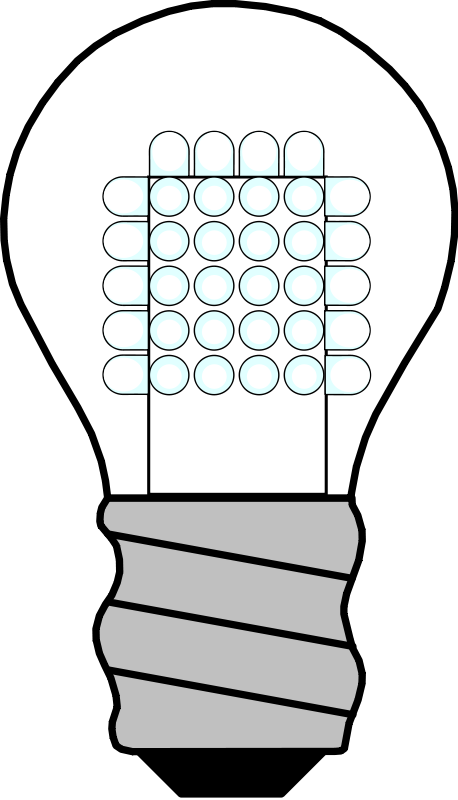
\includegraphics[scale=0.02]{imgs/bulb.png}
 \textbf{Nota} \\
 }%
{\endMakeFramed}

%Work in progress
\newenvironment{workinprogress}{%
  \def\FrameCommand{\colorbox{pink}}%
  \MakeFramed {\FrameRestore}
\lhdbend  \textbf{Work in progress} \\
 }%
{\endMakeFramed}

%Openquestion
\newenvironment{openquestion}{%
  \def\FrameCommand{\colorbox{pink}}%
  \MakeFramed {\FrameRestore}
 \textbf{Domanda aperta} \\
 }%
{\endMakeFramed}

%TODO
\newenvironment{todo}{%
  \def\FrameCommand{\colorbox{pink}}%
  \MakeFramed {\FrameRestore}
 \textbf{TODO} \\
 }%
{\endMakeFramed}

%%%%%%%%%%%%%%%%%%%%%%%%%%%%%%%%
%%%%%%%%%%%% HEADER %%%%%%%%%%%%
%%%%%%%%%%%%%%%%%%%%%%%%%%%%%%%%
\pagestyle{fancy}
% i comandi seguenti impediscono la scrittura in maiuscolo
% dei nomi dei capitoli e dei paragrafi nelle intestazioni
\renewcommand{\chaptermark}[1]{\markboth{#1}{}}
\renewcommand{\sectionmark}[1]{\markright{\thesection\ #1}}
\fancyhf{} % rimuove l'attuale contenuto dell'intestazione
% e del pi\`e di pagina
\fancyhead[LE,RO]{\bfseries\thepage}
\fancyhead[LO]{\bfseries\rightmark}
\fancyhead[RE]{\bfseries\leftmark}
\renewcommand{\headrulewidth}{0.5pt}
\renewcommand{\footrulewidth}{0pt}
\addtolength{\headheight}{0.5pt} % riserva spazio per la linea
\fancypagestyle{plain}{%
\fancyhead{} % ignora, nello stile plain, le intestazioni
\renewcommand{\headrulewidth}{0pt} % e la linea
}


%%%%%%%%%%%%%%%%%%%%%%%%%%%%%%%%
%%%%%%%%%%%% COLORS %%%%%%%%%%%%
%%%%%%%%%%%%%%%%%%%%%%%%%%%%%%%%
\definecolor{code}{gray}{0.3}


%%%%%%%%%%%%%%%%%%%%%%%%%%%%%%%%
%%%%%%%%%%%% NUMBERS %%%%%%%%%%%
%%%%%%%%%%%%%%%%%%%%%%%%%%%%%%%%
\setcounter{tocdepth}{3}
\setcounter{secnumdepth}{3}


%%%%%%%%%%%%%%%%%%%%%%%%%%%%%%%%
%%%%%%%%%%% DOC DATA %%%%%%%%%%%
%%%%%%%%%%%%%%%%%%%%%%%%%%%%%%%%
\title{Appunti di MNO}
\author{Gruppo Informatici Rampanti}
\date{ott 2010 - mag 2011}

\pdfinfo{%
  /Title    (Appunti di MNO)
  /Author   (Andrea Cimino e Lorenzo Muti)
  /Creator  (Andrea Cimino)
  /Producer (Lorenzo Muti)
  /Subject  (MNO)
  /Keywords (MNO)
}


%%%%%%%%%%%%%%%%%%%%%%%%%%%%%%%%
%%%%%%%%%%%%% UTILS %%%%%%%%%%%%
%%%%%%%%%%%%%%%%%%%%%%%%%%%%%%%%
% binary symbols
\newcommand{\modder}{\vdash _{R}}

% vertical gaps
\newcommand{\askip}{\vspace{0.5cm}}
\newcommand{\bskip}{\vspace{1.0cm}}

% various symbols
\newcommand{\qedhere}{\ensuremath{\Box}}
\newcommand{\qed}{\hfill \ensuremath{\Box}}

% substitution
\newcommand{\subst}[2]{^{#1} / _{#2}}

% denotational semantics function names
\newcommand{\bbracket}[1]{\left\llbracket #1 \right\rrbracket}

\newcommand{\aexpr}{\mathcal{A}}
\newcommand{\bexpr}{\mathcal{B}}
\newcommand{\cexpr}{\mathcal{C}}
\newcommand{\Aexpr}[1]{\mathcal{A} \bbracket{#1}}
\newcommand{\Bexpr}[1]{\mathcal{B} \bbracket{#1}}
\newcommand{\Cexpr}[1]{\mathcal{C} \bbracket{#1}}

\newcommand{\semdomset}[1]{(V_{#1})_{\bot}}

% semantic evaluations
\newcommand{\opereval}[3]{\left\langle #1, #2 \right\rangle \rightarrow #3}
\newcommand{\denaeval}[3]{\Aexpr{#1} #2 = #3}
\newcommand{\denbeval}[3]{\Bexpr{#1} #2 = #3}
\newcommand{\denceval}[3]{\Cexpr{#1} #2 = #3}

% rotated sqsubseteqs
\newcommand{\upsqsubseteq}{ $\begin{rotate}{90} $\sqsubseteq$ \end{rotate}$ }
\newcommand{\downsqsubseteq}{ $\begin{rotate}{270} $\sqsubseteq$ \end{rotate}$ }

% Space after paragraph declaration
\makeatletter
\renewcommand\paragraph{\@startsection{paragraph}{4}{\z@}%
  {-3.25ex\@plus -1ex \@minus -.2ex}%
  {1.5ex \@plus .2ex}%
  {\normalfont\normalsize\bfseries}}
\makeatother



% fast theorem and definition
\newcommand{\ftheo}[1]{\colorbox{YellowGreen}{#1}}
\newcommand{\fdefn}[1]{\colorbox{SkyBlue}{#1}}

\theoremstyle{break}
\theoremsymbol{\ensuremath{\clubsuit}}
\theoremseparator{\newline}
\newshadedtheorem{proc}[theo]{Procedura}

% bold math!
\newcommand{\bm}[1]{\mbox{\boldmath{$#1$}}}

\newcommand{\positive}[1]{\textbf{\color{green} +} #1}
\newcommand{\negative}[1]{\textbf{\color{red} -} #1}


\newtheoremlisttype{tab}%
{\begin{tabular*}{\linewidth}{@{}lrl@{\extracolsep{\fill}}r@{}}}%
{##1&##2&##3&##4\\}%
{\end{tabular*}}
\begin{document}
}
\providecommand{\outbpdocument}{\end{document}}
\else
\providecommand{\inbpdocument}{}
\providecommand{\outbpdocument}{}
\fi



\inbpdocument 

\chapter{Richiami di Algebra Lineare}

\section{Richiami su matrici}
Le matrici alle quali ci riferiremo saranno definite su campo dei complessi
 $\mathbb{C}$.\\
Lavoreremo quindi con dei vettori su
$\mathbb{C}$ : $v \in \mathbb{C}^h$, $A \in \mathbb{C}^{m \times n}$.

\subsection{Proprietà importanti sulle matrici}
\begin{defn}[Sottoinsieme chiuso rispetto alla moltiplicazione]
Un sottoinsieme di $C^{n\times n}$ si dice chiuso rispetto
all'operazione di moltiplicazione, se date due matrici $A$ e $B$ 
appartenenti al sottoinsieme, anche il
prodotto $AB$ appartiene al sottoinsieme. 
\end{defn}
I seguenti sottoinsiemi di
 $C^{n\times n}$ sono chiusi rispetto all'operazione di moltiplicazione:
\begin{itemize}
 \item matrici triangolari superiori (inferiori),
 \item matrici triangolari superiori (inferiori) in senso stretto
 \item matrici unitarie
\end{itemize} 
La moltiplicazione fra matrici gode della proprietà associativa, di quella
distributiva rispetto all’addizione, ma non di quella commutativa.

\begin{property}[Propriet\`a sul prodotto di matrici]
  \begin{itemize}
  \item  $A+ 0 = 0 + A = A$  (la matrice nulla \`e l'elemento neutro 
     della somma)
\item $ A+(-A) = 0$ (esistenza di un elemento opposto per la somma)
\item$ (A+ B) + C = A + (B+C)$ (propriet\`a associativa della somma)
\item $  A + B = B + A$   (propriet\`a commutativa della somma)
\item  $(AB)C = A(BC)$   (propriet\`a associativa del prodotto)
\item $ (A+B)C = AC + BC $ (propriet\`a distributiva)
\item $C(A+B) = CA + CB $  (propriet\`a distributiva)
 \end{itemize}
\end{property}

\begin{property}[Sull'inversione di matrici]
Vale la seguente propriet\`a:
$$ (AB)^{-1} = B^{-1} A^{-1}$$
\end{property}

Vale inoltre la seguente propriet\`a
\begin{property}[Reverse order law]
\begin{equation}\label{eq:eq001}  (AB)^{H} =  B^{H} A^{H}\end{equation}
dove $H$ \`e l'operatore di trasposizione coniugata.
\end{property}

\begin{openquestion}
Quali condizioni sono necessarie affinch\'e valga la reverse order law?
Una dimostrazione di tale proprietà: \\
si ponga 
$$ M = AB$$
Allora valgono le seguenti implicazioni
$$ A^{-1}M = A^{-1}AB \quad \Rightarrow \quad
 B^{-1}A^{-1}M = B^{-1}B  \quad
 \Rightarrow \quad
 B^{-1}A^{-1}M = I \quad 
$$
Ma allora $M$ deve essere l'inversa di $B^{-1}A^{-1}$, ma $M=AB$. \\
Il punto di questa dimostrazione che non mi \`e chiaro \`e:
quali condizione (ad esempio  sull'invertibilità di $A$ e $B$)
sono necessarie?

Ciuffo: Semplicemente che A e B siano invertibili, altrimenti 
l'operatore di inversa non dà risultati.
\end{openquestion}

\subsection{Alcune classi importanti di matrici}
\subsubsection{Matrici triangolari}
\begin{defn}[Matrice triangolare]
Le matrici triangolari inferiori (superiori) sono matrici quadrate che
hanno tutti gli elementi al di sopra (sotto) della diagonale
principale nulli.
\end{defn}

Il determinante di una matrice triangolare A può essere calcolato come il
prodotto dei sui elementi pricipali.
$$ \det(A) = \Pi_{i=1}^{n} a_{ii} $$ \label{triangolari}

\begin{defn}[Matrice Hessemberg]
\label{def:hessemberg}
Una matrice di Hessenberg \`e una matrice ``quasi'' triangolare. In
particolare \`e detta \emph{superiore} se ha valori pari a zero sotto la prima
sottodiagonale, viceversa nel caso \emph{inferiore}.
\end{defn}

\begin{example}[Hessemberg superiore e inferiore]
\[\begin{pmatrix}
  1 & 4 & 2 & 3 \\
  3 & 4 & 1 & 7 \\
  0 & 2 & 3 & 4 \\
  0 & 0 & 1 & 3 \\
\end{pmatrix}
\qquad
\begin{pmatrix}
  1 & 2 & 0 & 0 \\
  5 & 2 & 3 & 0 \\
  3 & 4 & 3 & 7 \\
  5 & 6 & 1 & 1 \\
\end{pmatrix}\]
\end{example}

\subsubsection{Matrici simmetriche}

\begin{defn}[Matrice simmetrica]
Una matrice simmetrica \`e una matrice quadrata che ha la proprietà di
essere uguale alla sua trasposta. Quindi A \`e simmetrica sse:
$$ A=A^T \qquad \text{cio\`e} \quad a_{ij} = a_{ji}, \; \forall i \forall j. \; a_{ij} \in A$$
\end{defn}

La classe delle matrici simmetriche \`e un sottoinsieme delle
 matrici Hermitiane.\\

\begin{defn}[Matrice trasposta coniugata]
Data una matrice $A \in C^{m \times n}$, si definisce matrice
trasposta coniugata di $A$ la matrice $B \in C^{n \times m}$ tale che
$$b_{ij} = \overline{a_{ji}}$$ 
dove $\overline{a_{ji}}$ \`e il coniugato del numero complesso $a_{ji}$,
e si indica
$$B = A^{H}$$
\end{defn}

\begin{defn}[Matrice Hermitiana]
Una matrice Hermitiana \`e una matrice a valori complessi che coincide
con la propria trasposta coniugata (o matrice aggiunta).
  $$ A = A^{H} $$
\end{defn}

Proprietà importanti di tali matrici:
\begin{itemize}
\item sulla diagonale principale \emph{devono} essere presenti solamente
  numeri reali. 
\item gli autovalori sono reali.
\item se $A$ \`e \emph{reale} hermitiana, allora risulta $A^{T} = A$ ed
\`e detta \emph{simmetrica}.
\end{itemize}

\begin{property}

Se $A \in  C_{n \times n}$ \`e una matrice hermitiana,
 cio\`e $A = A^{H}$, e $\mathbf{x} \in C_n$ , il  numero 
$$ \alpha =  \mathbf{x}^{H} A \mathbf{x}$$
\`e reale. Infatti, poich\'e  $A$ \`e hermitiana, si ha:
$$\overline{\alpha}  = \overline{\mathbf{x}^{H} A\mathbf{x}} =
 (\mathbf{x}^H A\mathbf{x})^H = 
 ((\mathbf{x}^H A)\mathbf{x})^H \underbracket{=}_{\ref{eq:eq001})} 
 \mathbf{x}^{H}(\mathbf{x}^{H}A)^{H} = 
\mathbf{x}^{H}(A^{H}\mathbf{x})=
 \mathbf{x}^H A^{H} \mathbf{x} = \mathbf{x}^H A\mathbf{x}  = \alpha.$$
\end{property}

\begin{example}[Matrice Hermitiana]
$$\begin{pmatrix}
  2   & 3+i \\
  3-i & 4
\end{pmatrix}$$
\end{example}

\subsubsection{Matrici unitarie}
\begin{defn}[Matrice unitaria]
  Una matrice $U$ \`e detta unitaria se soddisfa la condizione:
  $$U^H U = U U^H = I$$
  dove $I$ \`e la matrice identità.
\end{defn}

\paragraph{Proprietà}
\label{prop:unitarie}
\begin{itemize}
\item Dal punto di vista della complessità ottenere l'inversa
  di una matrice, che in generale ha costo cubico in n, per le
  unitarie \`e immediato, dato che $ U^{-1} = U^{H} $.
\item Le matrici unitarie hanno autovalori di modulo 1.
\item $U^{-1}$ \`e ancora una matrice unitaria.
\item Le matrici unitarie sono delle isometrie, o rispettano la norma
  2, ossia
  $$||Ux||_{2} = ||x||_{2}$$ 
  Infatti $|| Ux ||_{2} = \sqrt{x^{H}\underbracket{U^{H}U}_{I}x} = ||x||_{2}$
\item Le matrici unitarie danno garanzia di stabilità in tutti i
  calcoli in cui intervengono.
\item Se $A$ \`e \emph{reale} unitaria, allora $A^{T}A = AA^{T} = I$ ed
  \`e detta \emph{ortogonale}.
\end{itemize}

Inoltre le matrici unitarie su $\mathbb{R}^n$ sono tali che le loro colonne
formano una base ortonormale di $\mathbb{R}^n$, cio\`e per ogni coppia
di vettori della base il loro prodotto scalare \`e zero.\\
\begin{example}
  Ad esempio:
$$
\begin{bmatrix} 
  \cos \alpha & -\sin \alpha \\
  \sin \alpha & \cos \alpha
\end{bmatrix}
$$
\`e una base ortonormale di $\mathbb{R}^{2}$.
\end{example}

\begin{openquestion}
Queste considerazioni valgono anche per $\mathbb{R}$?

Ciuffo: certo che valgono anche per  $\mathbb{R}$: l'unica matrice
 unitaria per $\mathbb{R}$ \`e [1], quindi la proprietà
\`e banalmente dimostrata dato che non ci sono le coppie di colonne 
diverse della matrice per cui dovrebbe valere la proprietà.
\end{openquestion}

\paragraph{Matrici  unitarie importanti}
\subparagraph{Matrici di rotazione piana (2x2)}
Ruota un vettore di un angolo $\theta$
$$
G = 
\begin{bmatrix} 
\cos \theta & -\sin \theta \\
\sin \theta &  \cos \theta 
\end{bmatrix} 
$$

\subparagraph{Matrice di rotazione piana (n x n)}
$$ G =
\begin{bmatrix}
1 & 0 & 0 &...& ... &... & 0 & 0 & 0 \\
0 & 1 & 0 &... & ... &... & 0 & 0 & 0 \\
0 & 0 & ... & ... & ... &... & ...&0 & 0 \\
0 & 0 & ...  & cos(\theta ) &  ... & -sen(\theta ) & ... & 0&0 \\
0 & 0 & ... &  ... & 0 &... & ...& 0& 0 \\
0 & 0 & ... & 0 & 1 & 0 &...&0 &0\\
0 & 0 & ... & ... & 0 &... & ...& 0 & 0 \\
0 & 0 & ...  & sen(\theta ) &  ... & -cos(\theta ) & ...&0 &0 \\
0 & 0 & ... & ... & ... & ... & ...&0 & 0 \\
0 & 0 & 0 &... & ... & ... & 0 & 1 & 0 \\
0 & 0 & 0 &... & ... &... & 0 & 0 & 1 \\
\end{bmatrix}
$$

\subparagraph{Matrice di permutazione}
Una matrice di permutazione $P_{\pi}$, per la permutazione $\pi$ 
si ottiene da $I$ permutandone le righe.
\begin{example}[Matrice di permutazione]
  $$P_{\pi} =
  \begin{bmatrix}
    0 & 0 & 0 & 1  \\
    1 & 0 & 0 & 0  \\
    0 & 1 & 0 & 0  \\
    0 & 0 & 1 & 0  \\
  \end{bmatrix}
  $$
\end{example}

Dato che le matrici di permutazione sono matrici ortogonali, cio\`e
$P_{\pi}P_{\pi}^{T} = I$:

\begin{itemize}
\item sono matrici unitarie
\item l'inversa esiste e si scrive $P_{\pi}^{-1} = P_{\pi^{-1}} = P_{\pi}^{T}$
\end{itemize}

Nel caso di un vettore colonna $x$, $P_{\pi} x$ ne permuta le righe.

\subsection{Prodotto scalare}
\paragraph{su $\mathbb{R}^{n}$}
$$\langle u, v \rangle = \sum_{i=1}^{n} u_{i} v_{i} = u^{T}v$$

Si può inoltre definire la norma euclidea di un vettore tramite il
prodotto scalare in $\mathbb{R}^n$:
$$ || u || = \sqrt{\langle u,u \rangle} = \sqrt{\sum_{i=1}^{n} u_{i}^2} $$

\paragraph{su $\mathbb{C}^{n}$}
$$\langle u, v \rangle = \sum_{i=1}^{n} \overline{u_{i}} v_{i} = u^{H}v$$

Inoltre $u^{H} u = \sum_{i=1}^{n} \bar{u_i}u_i = \sum_{i=1}^{n} |
u_i|^{2}$ e quindi anche in questo caso basta fare la radice quadrata
per ottenere la norma euclidea.
\begin{property}\label{eigenvalues:ei001}
Il prodotto scalare $f(u,v)=\langle u,v \rangle$ su $\mathbb{C}^{n}$ gode
 delle seguenti proprietà:
\begin{itemize}
\item $f(au + bv, w) = af(u,w) + bf(v,w)$
\item $f(u,av + bw) = af(u,w)$
\item $f(u,v) = \overline{f(v,u)}$
\item $f(u,u) \geq 0$ \quad e 
       \quad  $f(u,u) = 0 \; \Longleftrightarrow \; u = 0$
\end{itemize}
\end{property}

Nota: il prodotto di un complesso per il suo coniugato ne dà il modulo
 al quadrato:
$$ (Re(\lambda) + i \; Im(\lambda)) \; (Re(\lambda) - i \; Im(\lambda)) = 
   Re^2(\lambda) + Im^2(\lambda)$$


\subsubsection{Matrici normali}
\begin{defn}[Matrice normale]
Una matrice quadrata $A$ \`e \emph{normale} se
$$ A^H A = A A^H $$
\end{defn}

Questa classe contiene anche le hermitiane e le unitarie, infatti:
\begin{itemize}
\item se una matrice \`e hermitiana allora \`e normale
\item se una matrice \`e unitaria allora \`e normale
\end{itemize}
\begin{property}
Una matrice normale pu\`o essere diagonalizzata per mezzo
di matrici unitarie.
\end{property}


\subsubsection{Matrici definite positive}
\begin{defn}[Matrice definita positiva]
Sia $A \in \mathbb{C}_{n\times n}$ una matrice hermitiana e 
sia $x \in \mathbb{C}_n , x \neq 0$.
Allora se il numero reale $x^{H} Ax > 0$ si dice che la matrice $A$ \`e
definita positiva.
Analogamente:
\begin{itemize}
\item se $x^{H} Ax \geq 0$, \quad A \`e semidefinita positiva
\item se $x^{H} Ax \leq 0$, \quad A \`e semidefinita negativa
\item se $x^{H} Ax < 0$, \quad A \`e definita negativa
\end{itemize}
\end{defn}

Sono una sottoclasse delle hermitiane.

\begin{property}
\label{prop:def-pos}
Una matrice $A^{H}A$ \`e semi-definita positiva.\\
Infatti $x^{H}A^{H} Ax =(Ax)^{H} Ax = || Ax|| \geq 0$
Se $A$ ha rango massimo allora $A^{H}A$ è definita positiva.
\end{property}


\subsubsection{Matrice partizionata a blocchi}
A volte \`e possibile dividere una matrice in sottomatrici o
\emph{blocchi}, e questo può agevolare delle operazioni come il
prodotto, che può essere ridefinito in termini del prodotto dei
blocchi.

\begin{example}[4 blocchi]
$$
\begin{array}{ll}
A = \left[
  \begin{array}{ccccc}
    & A_{11} & \vline & A_{12} \\
    \hline 
    & A_{21} & \vline & A_{22} \\
  \end{array}
\right]
&
B = \left[
  \begin{array}{ccccc}
    &  B_{11}& \vline & B_{12} \\
    \hline 
    & B_{21} & \vline & B_{22} \\
  \end{array}
\right]
\end{array}
$$

Prodotto:
$$
AB = \left[
  \begin{array}{ccccc}
    & A_{11}B_{11} + A_{12}B_{21} & \vline & A_{11}B_{12} + A_{12}B_{22} & \\
    \hline 
    & A_{21}B_{11} + A_{22}B_{21} & \vline & A_{21}B_{12} + A_{22}B_{22} &
  \end{array}
\right]
$$
\end{example}

Attenzione! I blocchi non sono commutativi! 


\subsubsection{Matrici riducibili}
\begin{defn}[Matrice riducibile]
Una matrice $A$ si dice riducibile se esiste una matrice di
permutazione $\Pi$ tale che
$$
B = \Pi \cdot A \cdot \Pi^{T} =
\left[ 
  \begin{array}{ccc}
    B_{11} & \vline & B_{12} \\ 
    \hline 
    O      & \vline & B_{22}
  \end{array}
\right]
$$
cio\`e con i blocchi diagonali $B_{11}$ e $B_{22}$ quadrati e $B_{21} = 0$.
\end{defn}

Questa proprieta \`e legata alla presenza di elementi nulli nella matrice di
 partenza $A$.\\
Pretendere che gli zeri siano sotto o sopra \`e arbitrario.\\

\paragraph{Matrici riducibili nella risoluzione di sistemi lineari}
Supponiamo $A$ riducibile: vogliamo risolvere il sistema di equazioni
$$Ax = b$$
Allora  
$$
\begin{array}{ll}
\Pi A x = \Pi b & \text{applichiamo permutazione} \\
\underbrace{\Pi A \Pi^{T}}_{B} \Pi x = \Pi b & 
\Pi \quad \text{\`e ortogonale, cio\`e} \quad \Pi \Pi ^{T} = I \\
B \Pi x = \Pi b & \text{ponendo} \quad \Pi x = y \quad \Pi b = c \\
B y = c
\end{array}
$$
Riscrivendo in forma matriciale, enfatizzando il fatto che si lavori
con matrici a blocchi:
$$
\left[
  \begin{array}{ccc}
    B_{11} & \vline & B_{12} \\
    \hline                    
    0      & \vline & B_{22}   
  \end{array}
\right]
\left[
  \begin{array}{c}
    y_1  \\
    \hline
    y_2 
  \end{array}
\right]
=
\left[
  \begin{array}{c}
    c_1  \\
    \hline
    c_2 
  \end{array}
\right]
$$
abbiamo triangolarizzato a blocchi la matrice senza fare calcoli.\\
Ora possiamo risolvere il seguente sistema lineare:
$$
\left\{
  \begin{array}{ll}
    B_{11}y_1 + B_{12}y_2 = c_1 \\
    B_{22}y_{2} = c_2           
  \end{array}
\right.
$$
Per riavere la soluzione originale basta riapplicare la permutazione
$x = \Pi^T y$ (costo zero).\\
Il costo totale di risolvere il nuovo sistema \`e $\frac{n^3}{12}$
contro il costo del normale metodo di Gauss $\frac{n^3}{3}$.

\begin{theo}
Una matrice \`e \emph{riducibile} sse il grafo associato non \`e fortemente
 connesso.
\end{theo}
Un grafo \`e fortemente connesso se da ogni nodo \`e possibile arrivare
 ad ogni altro nodo.
 
%% 29 Ottobre 2010
\section{Autovalori ed autovettori}
\begin{defn}[Autovalore/Autovettore]
\label{def:autovalore}
Siano $A \in \mathbb{C}^{n\times n}$, $x \in \mathbb{C}^{n}, x \neq 0$
e $\lambda \in \mathbb{C}$. Se vale 
$$ Ax = \lambda x $$ 
allora $x$ e $\lambda$ sono detti rispettivamente \emph{autovettore} e
\emph{autovalore} di $A$.
\end{defn}

\begin{defn}[Spettro di A]
Lo spettro di una matrice $A$ \`e costituito dall'insieme
degli autovalori di $A$
\end{defn}

\begin{defn}[Raggio spettrale di A]
Siano $\lambda_1, \ldots, \lambda_n \in \mathbb{C}$ gli autovalori di $A$. \\
Il raggio spettrale di $A$, denotato con $\rho(A)$, \`e 
definito come
$$ \rho(A) = \max_{i = 1, \ldots, n} | \lambda_i| $$ 
\end{defn}

\begin{defn}[Traccia di A]
Sia $A \in \mathbb{C}^{n\times n}$.
Si definisce \emph{traccia} di $A$ la quantit\`a
$$ tr(A) = \displaystyle \sum_{i=1}^{n} a_{ii}$$
\end{defn}

Valgono inoltre le seguenti propriet\`a
\begin{property}
$$ \displaystyle trA = \sum_{i=1}^{n} \lambda_i
\qquad
\displaystyle detA = \prod_{i=1}^{n} \lambda_i$$
\end{property}

Gli autovalori sono le soluzioni dell'
equazione caratteristica $p(\lambda) = 0$,
dove 
\begin{equation}
\label{eigenvalues:eq001}  p(\lambda) = det(A - \lambda I) =
 a_0 \lambda^{n} + a_1 \lambda^{n-1} +  \ldots + a_n 
\end{equation}
In particolare  vale la propriet\`a
\begin{property}
$$ a_1 = -(1)^{n-1}trA \qquad a_n= detA$$
\end{property}
Quindi il tutto può essere riscritto come
$$ p(\lambda)  =  (-1)^n\lambda^{n} + (-1)^{n-1}tr(A)^{n-1}+\ldots+det\; A $$
\`e il polinomio caratteristico di grado $n$. \\

Il problema degli autovalori \`e un problema non lineare e il grado del
polinomio cresce col crescere della dimensione della matrice.\\

Enunciamo inoltre un importante teorema, omettendone la dimostrazione.
Ci sar\`a utile in alcune dimostrazioni
\begin{theo}
  \label{eigenvalues:theo004}
  Una matrice $A$ di ordine $n$ \`e diagonalizzabile se e solo
  se ha $n$ autovettori linearmente indipendenti. Inoltre le colonne
  della matrice $S$, per cui $S^{-1}AS$ \`e diagonale, sono gli autovettori
  di $A$
\end{theo}

\begin{defn}[Sviluppo Laplace]
\label{sviluppo-laplace}
Lo sviluppo di Laplace \`e un metodo di calcolo del \emph{determinante}, che
risulta efficiente per matrici non troppo grandi e sparse. Si procede
scegliendo una riga, la $i$-esima, tramite la formula:

$$ \det(A) = \sum_{j=1}^n\ (-1)^{i + j} a_{i,j} \det(A_{ij}) $$

con $A_{ij}$ la matrice ottenura da $A$ eliminando la riga $i$-esima e la colonna
$j$-esima.

Esiste uno sviluppo analogo anche lungo la j-esima colonna.
\end{defn}


\paragraph{Matrici Hermitiane}
\begin{property}
Se $A$ Hermitiana allora gli autovalori sono reali $(\lambda \in \mathbb{R})$. 
\end{property}

\begin{thproof}
Usando la definizione di autovalore 
$$ Ax = \lambda x \quad \text{con} x \neq 0 $$
Calcolo la trasposta coniugata in entrambi i membri 
$$ x^H A^H = x^H \lambda^H= x^H \overline{\lambda} = \overline{\lambda} x^{H} $$
Moltiplico entrambi i membri per $x$ (diverso da 0 per ipotesi)
$$ x^H A^H x = \overline{\lambda}  x^{H} x \qquad (1) $$
Prendo la definizione di autovalore e moltiplico entrambi i membri per $x^{H}$
$$x^{H} A x = x^{H} \lambda x = \lambda x^{H} x \qquad (2)$$
Dato che A \`e hermitiana (1) e (2) sono uguali, da cui
$$ \lambda x^{H} x = \overline{\lambda} x^{H} x$$
Dato che $x^{H} x \neq 0 \; (\sum |x_i|^{2} \neq 0) $ allora posso
 semplificare, ottenendo
$$ \lambda=\overline{\lambda} \; \Rightarrow \; \lambda \in \mathbb{R} $$
\end{thproof}


\paragraph{Matrici Unitarie}
Verifichiamo gli autovalori per le matrici unitarie:
\begin{property}
Sia $U$ unitaria allora i suoi autovalori hanno modulo 1.
 $$| \lambda | = 1 $$
\end{property}

\begin{thproof}
Sia $\lambda$ un autovalore. Poich\'e per le matrici unitarie vale la
propriet\`a
$$ |Ux| = |x|$$
inoltre vale per definizione
$$  U^{H} U = I$$
Moltiplicando ciascun membro di $Ux = \lambda x$ per se stesso trasposto
 coniugato, usando la reverse order law ({\ref{eq:eq001})}, otteniamo
$$ x^{H} \underbracket{U^{H} U}_{I}x = x^{H}x \overline{\lambda} \lambda 
\quad 
\Rightarrow 
 \quad \underbracket{x^{H}x}_{scalare} = |\lambda|^2 \underbracket{x^{H}x}_{\text{scalare}}  
 \quad \Rightarrow \quad  1 = | \lambda|^{2}$$
\end{thproof}


\paragraph{Autovalori per matrici definite positive}
\begin{property}
$A$ è definita positiva se e solo se
i suoi autovalori sono reali positivi.
\end{property}

\begin{thproof}
Al solito prendiamo la definizione di autovalore
$$ Ax = \lambda x$$
Moltiplicando i due membri per $x^{H}$ a sinistra
$$ x^{H}Ax = x^{H} \lambda x$$
che \`e equivalente a
$$ x^{H}Ax =  \lambda x^{H}  x$$
Utilizzando per ipotesi
\begin{itemize}
\item $x^{H}x > 0 $ per una delle (\ref{eigenvalues:ei001})
\item $x^{H}Ax > 0$ essendo $A$ definita positiva
\end{itemize}
possiamo scrivere
$$ \underbracket{x^{H}Ax}_{>0} =  \lambda \underbracket{x^{H}x}_{>0}$$
Ma allora $\lambda$ deve essere necessariamente positivo
\end{thproof}

Quindi definita positiva implica tutti gli autovalori positivi e vale
anche il viceversa anche se dobbiamo dimostrarlo.\\

\begin{theo}[Definite positive e loro principali di testa]
\label{richiamibevilacqua:definitepositive}
Una matrice hermitiana A \`e definita positiva se e solo se i
determinanti di tutte le sottomatrici principali di testa di A (e quindi anche
il determinante di A) sono positivi.
\end{theo}

\begin{defn}
  Sottomatrici principali sono quelle matrici create scegliendo
  colonne e righe con gli stessi indici.
\end{defn}

\begin{example}
  Prendendo gli indici 1 e 3 da una matrice 4 x 4 otteniamo una
  sottomatrice principale 2x2 con la diagonale sovrapposta a quella
  della matrice di origine.
\end{example}

%%% Warning: Dimostrazione??? 


\begin{theo}[Teorema di Cayley - Hamilton]
\label{eigenvalues:teo01} 
 Sia $p$ il polinomio caratteristico di $A$ allora
 $$ p(A) = 0$$
\end{theo}
\begin{thproof}
 (Rimandiamo la dimostrazione, quando si parler\`a di diagonalizzazione) 
\end{thproof}
Vediamo per $n = 2$ \\
Il polinomio caratteristico \`e dato da
$$ p(\lambda) = (-1)^{2} \lambda^{2} - tr(A)\cdot \lambda + detA $$
Allora il teorema afferma che per ogni matrice $A$ vale
$$p(A) = A^2 - tr(A) \cdot \lambda + det\; A \cdot I \underbracket{ = 0
} $$
Non \`e ovvio che quello sia 0, \`e quindi un teorema importante.
 \\ \\
Vediamo nel caso $A \quad m \times n$
\begin{equation}
\label{eigenvalues:eq002} 0 = a_{0}A^{n} + a_1 A ^{n-1} \ldots a_{n}I  =  p(A)
\end{equation}
Se $A$ \`e invertibile, moltiplicando per $A^{-1}$ otteniamo
$$ 0 = a_0 A^{n-1} + a_1 A^{n-2} \quad \underline{a_n}A^{-1}$$
$a_n \neq 0$ perch\`e sappiamo che \`e il determinante, quindi
$$ A^{-1} = \frac{1}{a_n}\cdot \left( \text{polinomio in A di grado n-1} \right) $$
\begin{openquestion}
Come \`e stata fatta questo accenno alla matrice inversa?
Cosa si voleva fare vedere? Si voleva fare vedere per
caso che $1/a_{n}$ \`e un autovalore di $A^{-1}$
\end{openquestion}
Non serve considerarare polinomi in una matrice di grado troppo elevato
 (maggiore o uguale a $n$) \\
Sia $S$ un polinomo di grado $m \geq n$ dove $n$ \`e l'ordine della matrice.
Allora 
$$ \underbracket{S(x)}_{m}  = \underbracket{p(x)}_{n}\underbracket{q(x)}_{m-n} + \underbracket{r(x)}_{< n} \quad \text{divisione fra polinomi} $$
$$S(A) = \underbracket{\cancel{p(A) q(A)}}_{=0 \;(\ref{eigenvalues:teo01})} + r(A) = 0$$
Quindi abbiamo un polinomio di grado $< n$ \\
C'\`e un polinomio (polinomio minimo): \`E possibile che esistano altri
 polinomi $S(\lambda)$
con $S(A) = 0$ e grado minore di $n$
\begin{defn}[Polinomio minimo]
Si definisce polinomio minimo $\psi(\lambda)$ il polinomio monico 
(ossia con primo coefficiente uguale a 1) di grado minimo tale che
 $\psi(A) = 0$ (matrice nulla)
\\ From Wikipedia\\ \\
Data una matrice quadrata $A$ a valori in un certo campo $K$, si considera
l'insieme $$ I = \{p\in K[x]\ |\ p(A) = 0\} $$
di tutti i polinomi che annullano $A$. Questo insieme risulta essere
un ideale nell'anello $K[x]$ di tutti i polinomi con coefficienti in $K$.
\\ \\
L'anello $K[x]$ \`e un anello euclideo: \`e infatti possibile fare una
divisione fra polinomi con resto. Conseguentemente, \`e un anello ad
ideali principali: ogni ideale \`e generato da un unico elemento. 
In particolare, :$I = (m(x))\,\!$ 
\`e generato da un elemento $m(x)$. Tale elemento \`e unico solo a meno 
di moltiplicazione per una costante non nulla: \`e quindi unico se lo si 
suppone ''monico'' (cio\`e con coefficiente 1 nel termine $x^k$ più grande).
Si definisce quindi il '''polinomio minimo''' di $A$ tale polinomio $m(x)$.
\end{defn}
\begin{example}
 $$A = I_{n} $$
 $$ P(\lambda ) = (1-\lambda)^{n} \qquad  det(I - \lambda I) = 
\left[
\begin{array}{cc}
 ( 1 - \lambda  & 0 \\
0   & 1-\lambda)
\end{array}
\right]
 $$
 $$ \psi(\lambda) = -(1 -\lambda) = \lambda -1 $$
$$ \psi(I) = I - I = 0$$           
\end{example}
\begin{example}
 From Wikipedia \\
Consideriamo per esempio la matrice 
$$A = \begin{bmatrix}1&2\\
3&4\end{bmatrix}$$
Il suo polinomio caratteristico \`e dato da

$$p(\lambda)=\det\begin{bmatrix}1-\lambda&2\\
3&4-\lambda\end{bmatrix}=(1-\lambda)(4-\lambda)- 2\cdot 3=\lambda^2-5\lambda-2.$$
Il teorema di Cayley–Hamilton sostiene che:
$$A^2-5A-2I_2=0\,\!$$
il che si può facilmente verificare.
\end{example}

\section{Forme canoniche}
\begin{defn}[Matrici simili]
Due matrici quadrate $A$ e $B$ si dicono simili
se esiste una matrice $M$ invertibile per cui vale
$$ A = M^{-1}BM$$
\end{defn}
\`e facile verificare quindi che la similitudine fra matrici
\`e una relazione di equivalenza nell'insieme delle matrici
$M_{n \times n}$
\begin{property}
Matrici simili godono delle seguenti propriet\`a:
\begin{itemize}
 \item hanno stesso rango;
 \item hanno stessa traccia;
 \item hanno stesso determinante;
 \item hanno stesso polinomio caratteristico: questo implica
       che due matrici simili hanno stessi autovalori.
\end{itemize}
\end{property}

\begin{defn}[Molteplicit\`a algebrica e geometrica]
Sia $\lambda_i$ un autovalore di una matrice $A$.\\
Diremo \emph{molteplicit\`a algebrica} di $\lambda_i$
la sua molteplicit\`a nel poliniomo caratteristico. \\
Diremo inoltre \emph{molteplicit\`a geometrica} di $\lambda_i$
la dimensione del relativo autospazio $V_{\lambda_i}$
\end{defn}
Da ricordarsi che una matrice \`e diagonalizzabile se e solo
se molteplicit\`a algebrica e geometrica coincidono. Se non fosse
così, ricordando che la molteplicit\`a algebrica \`e sempre
maggiore o uguale a quella geometrica, possiamo cercare di ricondurre
una data matrice, ad una matrice che abbia una struttura simile
a quella di una matrice diagonale, ed \`e detta forma canonica
di Jordan. Ogni matrice quadrata \`e riconducibile a forma
di Jordan.

\subsection{Forma canonica di Jordan}
La forma canonica di Jordan di una matrice quadrata $A$ definisce una
matrice triangolare $J$ \emph{simile} ad $A$ che ha una struttura il
più possibile vicina ad una matrice diagonale. La matrice \`e diagonale
se e solo se A \`e diagonalizzabile, altrimenti \`e divisa in blocchi
detti blocchi di Jordan.\\

La forma canonica caratterizza univocamente la classe di similitudine
di una matrice, cio\`e due matrici sono simili se e solo se hanno la
stessa forma di Jordan (a meno di permutazione dei blocchi).\\

\paragraph{Blocco di Jordan}
Un \emph{blocco di Jordan} di ordine $k$ \`e una matrice triangolare
superiore con $k$ righe costituita nel seguente modo:
$$
\begin{pmatrix}
 \lambda & 1      & 0      & \cdots & 0      \\                       
 0       & \ddots & \ddots &        & \vdots \\
 \vdots  & \ddots & \ddots & \ddots & 0      \\
 \vdots  &        & \ddots & \ddots & 1      \\
 0       & \cdots & \cdots & 0      & \lambda    
\end{pmatrix}
$$

in cui ogni elemento della diagonale \`e uguale a $\lambda$ ed in ogni
posizione (''i'', ''i''+1) si trova un 1. Il suo polinomio
caratteristico \`e $ (x-\lambda)^k $, e quindi ha $\lambda$ come unico
autovalore con molteplicit\`a algebrica $k$.      \\
D'altra parte, l'autospazio relativo a $\lambda$ \`e:
$$ \ker(J_k(\lambda) - \lambda I) = \ker\begin{pmatrix}
 0      & 1      & 0      & \cdots & 0          \\                       
 0      & \ddots & \ddots &        & \vdots     \\
 \vdots & \ddots & \ddots & \ddots & 0          \\
 \vdots &        & \ddots & \ddots & 1          \\
 0      & \cdots & \cdots & 0      & 0    
\end{pmatrix} = \textrm{Span} \begin{pmatrix} 1 \\ 0 \\ \vdots \\ \vdots \\ 0 \end{pmatrix} $$
avente, quindi, dimensione 1. Dal teorema di diagonalizzabilit\`a segue che se 
$k>1$ il blocco di Jordan non \`e diagonalizzabile.

\paragraph{Matrice di Jordan}
Una matrice di Jordan \`e una matrice a blocchi del tipo
\[ J = 
\begin{pmatrix} 
  J_1 &        & 0 \\ 
      & \ddots &   \\ 
  0   &        & J_k 
\end{pmatrix} 
\]

dove $J_i$ \`e un blocco di Jordan con autovalore $\lambda_i$. Ogni
blocco di Jordan contribuisce con un autospazio unidimensionale
relativo a $\lambda_i$.\\
\begin{itemize}
\item La molteplicit\`a geometrica di $\lambda_i$, definita come la
  dimensione del relativo autospazio, \`e pari al numero di blocchi con
  autovalore $\lambda_i$.
\item La molteplicit\`a algebrica di $\lambda_i$, definita come la
  molteplicit\`a della radice $\lambda_i$ nel polinomio caratteristico di
  $J$, \`e pari alla somma degli ordini di tutti i blocchi con autovalore
$\lambda_i$.
\end{itemize}
Il teorema di diagonalizzabilit\`a asserisce che $J$ \`e diagonalizzabile
se e solo se le molteplicit\`a algebriche e geometriche coincidono,
ovvero se e solo se i blocchi hanno tutti ordine pari ad 1: in altre
parole, $J$ \`e diagonalizzabile se e solo se \`e gi\`a diagonale.


\begin{example}[Esempio da Wikipedia]
Calcoliamo la forma canonica di Jordan della matrice 

$$A =
\begin{pmatrix}
 5 &  4 &  2 &  1 \\
 0 &  1 & -1 & -1 \\
-1 & -1 &  3 &  0 \\ 
 1 &  1 & -1 &  2 \\
\end{pmatrix}$$

Il suo polinomio caratteristico \`e $$ (x-4)^2(x-2)(x-1) $$ Quindi i suoi
 autovalori sono 4, 4, 2 e 1. Ricordiamo che, se indichiamo con
 $m_{alg}(\lambda)$ e
$m_{geo}(\lambda)$ le molteplicit\`a algebrica e geometrica di un autovalore
$\lambda$ valgono sempre le seguenti disuguaglianze:

$$ 1 \leq m_\textrm{geo}(\lambda) \leq m_\textrm{alg}(\lambda) $$

Quindi in questo caso le molteplicit\`a algebriche e geometriche degli autovalori
 2 e 1 sono tutte 1, e l'unica grandezza da trovare \`e la molteplicit\`a
geometrica di 4, che può essere 1 o 2. La molteplicit\`a geometrica di un
autovalore indica il numero di blocchi di jordan presenti relativi a 
quell'autovalore. Vediamo che

$$ \dim\ker (A-4I) = 1. $$

Segue quindi che ''A'' non \`e diagonalizzabile, e l'autovalore 4 ha un solo
blocco di Jordan. I dati che abbiamo sono sufficienti a determinare la matrice
 di Jordan, che \`e la seguente:

$$J=\begin{pmatrix}
4 & 1 & 0 & 0 \\
0 & 4 & 0 & 0 \\
0 & 0 & 2 & 0 \\
0 & 0 & 0 & 1 \end{pmatrix}$$
\end{example}

%%%%%%%%%%%%%%
% NICOLA: Commento perche' questa parte
% e' scorrelata dal resto...
%Se $B$ \`e  $\left\{
%\begin{array}{l}
% \text{diagonale (a blocchi)} \\
% \text{triangolare (a blocchi)}
%\end{array}
% \right.
%$

Forma canonica di Jordan:
Qualunque matrice A \`e riconducibile a forma canonica di Jordan
$$S^{-1} A S =J $$
\begin{example}[Esempio visto a lezione]
Prendiamo il caso $n = 9$ , con i seguenti autovalori:
$$
\left\{
\begin{array}{cc}
 \lambda_1 = 2  & \text{ con molteplicit\`a algebrica } 5
,\text{ geometrica  2 }\\
\lambda_2 = 3   & \text{ con molteplicit\`a algebrica } 2
,\text{ geometrica  1 } \\
\lambda_3 = 1   & \text{ con molteplicit\`a algebrica } 2
,\text{ geometrica  2 } 
\end{array}
\right.
$$

Allora la forma canonica prende gli autovalori distinti
La matrice di Jordan sar\`a composta dai seguenti blocchi
$$ J =
\left[
\begin{array}{ccc}
B_{5 \times 5} & 0 & 0 \\ 
0 & B_{2 \times 2}  & 0 \\
0 & 0 & B_{2 \times 2} \\
\end{array}
\right]
$$
$$
J = 
\left[
\begin{array}{cccccccccc}
2& 1& & & & & & \multicolumn{3}{c}{\multirow{4}{*}{\Huge $0$}}
 \\
& 2 & 1 & & & & & & \\
& &2& 1 & & & & & & \\
& & & 2 & & & & & & \\
& & & &2 & 1 & & & & \\
& & & & & 2 & & & & \\
& & & & & & 3 & 1 & & \\
\multicolumn{3}{c}{\multirow{4}{*}{\Huge $0$}}
& &  & & & 3 & & \\
& & & & & & & & 1& \\
& & & & & & & & & 1 \\
\end{array}
\right]
$$

Polinomio caratteristico :
$$
\underbracket{p(\lambda) = (\lambda -2)^{5} (\lambda -3)^{2} (\lambda -1)^2}_{checkme!!}$$
Questo non dice come spaccare il blocco più grande i blocchi più piccoli.
(3,2) (4,1) etc \ldots. \\
Adesso \`e facile verificare il teorema di Caley Hamilton perch\'e
$$p(A) = p(\underbracket{SJS^{-1}}_{\text{diagonale a blocchi}})$$
$$ S^{-1} A S = J$$
$$a_0(SJS^{-1})^{2} + a_1 (SJS^{-1}) + a_2 I$$
$$ SJ^{2}S^{=1}      a_1(SJS^{-1}) + a_2 S S^{-1} = S p(j) S^{-1}$$
I polinomi dei singoli blocchi fanno zero.\\
Prendiamo il primo blocco e lo chiamiamo $C$.

$$p(C) = (-1)^{9}$$
$$(C -2I)^{5}(C-3I)^{2}(C-I)^{2} $$
\begin{notes}
CHECKME
\end{notes}

Se svolgiamo  
\begin{Verbatim}
                         ^5
	        0   1  0 
 (C -2I)^{5} =  0  0   1    = 0
		0  0   0  
\end{Verbatim}

$\sigma(\lambda_i) \geq \text{ dimensione del blocco }$\\
Basta che si annulli una delle componenti di sopra anche il prodotto 
totale sia 0.
\end{example}

\begin{theo}
La forma canonica di Jordan \`e diagonale (a elementi)  (A \`e diagonalizzabile)
se e solo se
esistono  $n$ autovettori linearmente indipendenti.
\end{theo}
Caso particolare: poich\'e  ad autovalori distinti corrispondono autovettori
linearmente indipendenti, quindi se $A$ possiede $n$ autovalori distinti\
allora \`e diagonalizzabile.

\subsection{Forma canonica di Schur}

\begin{theo}[Forma canonica di Schur]
\label{eigenvalues:schur}
Sia $A \in \mathbb{C}^{n\times n}$ e siano $\lambda_1, \ldots, \lambda_n$
i suoi autovalori. Allora esiste una matrice unitaria $U$ e 
una matrice triangolare superiore $T$ i cui elementi principali sono
i $\lambda_i$, tali che
$$ A = UTU^{H} $$
\end{theo}

$T=U^{H}AU$ \`e detta \emph{forma di Schur} di $A$.\\ 
Dato che $T$ 
\begin{itemize}
\item \`e simile ad $A$, ha gli stessi autovalori 
\item \`e triangolare, ha gli autovalori lungo la diagonale.
\end{itemize}
Inoltre ricordiamo che essendo $U$ unitaria, $U^{H} = U^{-1}$.

\begin{notes}
 La dimostrazione \`e copiata pari pari dal libro del professore.
\end{notes}

\begin{thproof}
Si procede per induzione. Per $n=1$ la tesi vale con $U = [1]= a_{11}$. \\
 per $n>1$, sia $x_1$ l'autovettore normalizzato
corrispondente all'autovalore $\lambda_1$ e sia $S$ lo spazio
generato da $x_1$. Indicata con $y_2, \ldots, y_n$ una base
ortornormale dello spazio $S^{\bot}$, la matrice
$$ Q = [ x_1 | y_2 | \ldots | y_n ] $$
\`e unitaria e $Q^{H}x_1 = e_1$. Si considera la matrice
$$ B = Q^{H}AQ$$
la cui prima colonna \`e
$$ Be_1 = Q^{H}AQe_1 = Q^{H}Ax_1 = Q^{H}\lambda_1 x_1 = 
\lambda_1 Q^{H}x_1 = \lambda_1 e_1$$
e qindi $B$ può essere partizionata nel seguente modo:
$$
B =
\left[
\begin{array}{ccc}
\lambda_1 & & c^{H}  \\
& & \\
0 & & A_1 
\end{array}
\right]
$$
dove $c \in \mathbb{C}^{n-1}$ e $A_1 \in \mathbb{C}^{(n-1)\times (n-1)}$.
Per l'ipotesi indutiva esiste una
 matrice unitaria $U_1 \in \mathbb{C}^{(n-1)\times (n-1)}$. tale che
$$ A_1 = U_1 A_2 U_1^{H} $$
dove $A_2 \in \mathbb{C}^{(n-1)\times (n-1)}$ \`e triangolare superiore.
Allora risulta
$$ A = QBQ^{H} = Q
\left[
\begin{array}{ccc}
\lambda_1 & & c^{H}  \\
& & \\
0 & & A_1 
\end{array}
\right]
Q^{H} =
 Q 
\left[
\begin{array}{ccc}
\lambda_1 & & c^{H}  \\
& & \\
0 & & U_1A_2U_1^{H} 
\end{array}
\right]
Q^{H}
$$
Indicando con $U^{2} \in \mathbb{C}^{m \times n}$ la matrice unitaria
$$ U_2 =
\left[
\begin{array}{ccc}
1 & & 0^{H}  \\
& & \\
0 & & U_1 
\end{array}
\right]
$$
si ha:
$$ A = QU_2
\left[
\begin{array}{ccc}
\lambda_1 & & c^{H}U_1  \\
& & \\
0 & & A_2 
\end{array}
\right]
U_2^{H}Q^{H}
$$
Poich\'e la matrice $U=QU_2$ \`e ancora unitaria in quanto 
prodotto di matrici unitaria, risulta
$$ A = U
\left[
\begin{array}{ccc}
\lambda_1 & & c^{H}U_1  \\
& & \\
0 & & A_2 
\end{array}
\right]
U^{H}
$$
da cui la tesi, essendo $A_2$ matrice triangolare superiore.
\end{thproof}


%% 2 Novembre 2010
\begin{notes}
 Il professore ha enunciato la seguente proprieta:\\
Se A \`e Hermitiana e applichiamo il Teorema di Schur, T risulta
diagonale. \\
La dimostrazione \`e stata abbozzata, e qui la ripropongo
in versione completa, come dal libro
\end{notes}
% 
% Anche $T$ risulta essere Hermitiana, infatti $T$, dal teorema di
% Schur
%  $$ T = U^{H}AU \qquad T^{H} = (U^{H}AU)^{H} = U^{H}A^{H}(U^{H})^{H} = U^{H}AU = T$$
% T.Superiore
% --------
% -
%   - 
% 0-   - 
% --------
%    
%  = 
% --------
% -     0
%   - 
%      - 
% --------   
% Allora T \`e diagonale
% 
% Le matrici herminiane sono tutte diagonalizzabili unitarie.
% 
% $$U^{H}AU = T = 
% \begin{pmatrix}
% \lambda_1& 0 +i\\
% 0 & \lambda_n  
% \end{pmatrix}
%  $$

\begin{theo} \label{eigenvalues:theo005}
 Sia $A$ una matrice hermitiana di ordine $n$, cio\`e
$A = A^{H}$ e siano $\lambda_1, \ldots, \lambda_n$ i suoi
autovalori. Allora esiste una matrice unitaria $U$
tale che
$$ A = U
\left[
\begin{array}{cccc}
\lambda_1 & & &  \\
& \lambda_2 & &  \\
 & & \ddots &  \\
 & &  & \lambda_n 
\end{array}
\right]
U^{H}
$$
\end{theo}


\begin{thproof}
Per il teorema \ref{eigenvalues:schur} si ha $T = U^{H}AU$, dove $T$ \`e 
una matrice triangolare superiore e $U$ \`e unitaria. Poich\'e $A =A^{H}$, si ha
$$ T^{H} = (U^{H}AU)^{H} = U^{H}A^{H}U = U^{H}AU = T$$
cio\`e la matrice triangolare $T$ risulta essere una matrice
diagonale con gli elementi principali reali e per il teorema
\ref{eigenvalues:theo004} le colonne di $U$ , che sono ortonormali perch\'e $U$
\`e unitaria, risultano essere gli autovettori di $A$
\end{thproof}

\begin{notes}
 Anche il seguente teorema e dimostrazione \`e copiato pari pari
dal libro, poich\`e i passaggi sono molto più chiari.
\end{notes}

\begin{theo}
Una matrice $A \in \mathbb{C}^{n\times n}$ \`e normale, cio\`e
$A^{H}A = AA^{H}$, se e solo esiste una matrice unitaria $U$ tale che
$$ A = U
\left[
\begin{array}{cccc}
\lambda_1 & & &  \\
& \lambda_2 & &  \\
 & & \ddots &  \\
 & &  & \lambda_n 
\end{array}
\right]
U^{H}
$$
 Le matrici normali  $(A^{H}A = AA^{H})$
 sono tutte e sole quelle diagonalizzabili con $U$ unitaria 
 $$ A= UDU^{H}$$
\end{theo}
\begin{thproof}
 $\Longrightarrow$:
Si supponga dapprima che $A$ sia normale. Per il teorema
\ref{eigenvalues:schur}
esiste una matrice $U$ unitaria tale che
$$T = U^{H}AU$$
con $T$ matrice triangolare superiore e si ha:
$$ T^{H}T = U^{H}A^{H}UU^{H}AU = U^{H}A^{H}AU \qquad
TT^{H} = U^{H}AUU^{H}A^{H}U = U^{H}AA^{H}U $$
Poich\'e $A$ \`e normale, ne segue che
\begin{equation}
\label{eigenvalues:equ004}
 T^{H}T = TT^{H}
\end{equation}
e quindi anche $T$ \`e normale. Si dimostra per induzione su $n$
che $T$ \`e diagonale. Se $n=1$ questo \`e ovvio. Se
$n>1$, poich\'e $T$ \`e triangolare superiore, per l'elemento $p_{11}$
della marice $P=T^{H}T = TT^{H}$, si ha
$$p_{11} = \overline{t_{11}}t_{11} = | \lambda_1|^{2} 
\qquad \text{e} \qquad
p_{11} = \displaystyle \sum_{j=1}^{n} 
 t_{1j}\overline{t_{1j}} = |\lambda_1|^{2} + 
\displaystyle \sum_{j=2}^{n} |t_{1j}|^{2} $$
da cui
$$ t_{1j}=0, \qquad \text{per } j=2, \ldots, n$$
cio\`e la prima riga di $T$ ha tutti gli elementi nulli eccetto quello
principale. Indicata con $T{n-1}$ la sottomatrice ottenuta da $T$
cancellando la prima riga e la prima colonna dalla (\ref{eigenvalues:equ004})
segue che
$$T_{n-1}^{H} T_{n-1} = T_{n-1}T_{n-1}^{H}$$
Per l'ipotesi induttiva $T_{n-1}$ \`e diagolnale, e quindi
$T$ risulta diagonale.
\end{thproof}

\section{Alcune propriet\`a delle matrici definite positive}
 $$ x^{H}Ax > 0 \quad \text{ per } x\neq 0 $$ 
Ricordiamo le propriet\`a:
\begin{itemize}
 \item $A$ definita positiva $ \Longleftrightarrow $ tutti gli autovalori di $A$ sono reali positivi.
 \item $A$ definita positiva $ \Longleftrightarrow $  le sottomatrici principali di testa
hanno determinante positivo.
\end{itemize}
\begin{notes}
 Qui il professore ha enunciato il seguente teorema, dimostrandone a
 lezione solo un verso.
\end{notes}

\begin{theo}
\label{eigenvalues:theo006}
 Sia $A$ una matrice hermitiana di ordine $n$ e siano
$\lambda_1, \ldots, \lambda_n$ i suoi autovalori. Allora
$A$ \`e definita positiva se e solo se $\lambda_i > 0, i =1, \ldots n$.
\end{theo}
\begin{thproof}
Vediamo l'implicazione contriaria ossia
autovalori reali positivi sono quelle definite positive
e questo lo vediamo con Schur. (la freccia opposta del primo punto). \\
Poich\'e $A$  \`e hermitiana, risulta
$$ A = UDU^{H}$$ 
con $U$ matrice unitaria e $D$ matrice diagonale avente come elementi principali
gli autovalori $\lambda_i, i=1, \ldots,n$ di $A$. Se $x \in \mathbb{C}^{n}, x \neq 0$,
si ha
\begin{equation}
\label{eigenvalues:equ005}
x^{H} A x = x^{H}UDU^{H}x = y^{H}Dy 
\end{equation}

dove il vettore $y = U^{H}x$ non può essere uguale a $0$, perch\'e $U$
non \`e singolare. Dalla (\ref{eigenvalues:equ005}) si ha:
$$ 
\begin{array}{c}
x^{H}Ax = (\overline{y}_1, \ldots, \overline{y}_n)
 \left[
\begin{array}{cccc}
\lambda_1 & & &  \\
& \lambda_2 & &  \\
 & & \ddots &  \\
 & &  & \lambda_n 
\end{array}
\right]
\left[
\begin{array}{c}
y_1 \\
\vdots \\
y_n
\end{array}
\right]
 = \overline{y_{1}}\lambda_1 y_1 + \overline{y_{2}}\lambda_2 y_2 +
   \ldots + \overline{y_{n}}\lambda_n y_n = \\
 = \displaystyle \sum_{i=1}^{n} \underbracket{|y_i|^{2}}_{\geq 0} \underbracket{\lambda_{i}}_{>0}
 > 0
\end{array}
$$
poich\`e gli autovalori $\lambda_i$ sono tutti positivi e gli $|y_i|$
sono tutti non nulli.
\begin{notes} 

 Non ho segnato e capito perch\`e l'ultimo passaggetto \`e > 0 \\
Ciuffo: dai miei appunti ho che:  il caso = 0 si ha quando ogni $y_{i} = 0$,
quindi l'intero vettore y dev'essere 0, 
ma dato che $ y=U^{H}x $ e che per ipotesi di A definita positiva abbiamo
 $ x \neq 0 $, e dato che U \`e unitaria, 
allora esiste un $ y_i > 0 $ che rende la sommatoria > 0 .
Di questa spiegazione va inserita la versione in italiano
\end{notes}
\end{thproof}

\section{Localizzazione degli autovalori}
\begin{defn}[Cerchi di Gerschgorin]
Sia $A \in \mathbb{C}^{m \times n}$. I cerchi del piano complesso
 $$K_i = \{ z \in \mathbb{C} :  \quad  |z - a_{ii}| \leq 
\displaystyle \sum_{j=1 \\ j\neq i}^{n} |a_{ij}| \}, i = 1,2, \ldots, n
$$ 
di centro $a_{ii}$ e raggio $r= \displaystyle\sum_{j=1 ~ j\neq i}^{n} |a_{ij}|$ 
sono detti \emph{cerchi di Gershgorin}.
\end{defn}



\begin{theo}[Primo teorema di Gershgorin]
Gli autovalori della matrice $A$ di ordine $n$ sono tutti contenuti in
$$ \displaystyle \bigcup_{i= 1, \ldots, n} K_{i}$$
\end{theo}


\begin{theo}[Terzo teorema di Gershgorin]
Se la matrice $A$ di ordine $n$ \`e irriducibile, ogni autovalore $\lambda$,
che sta sulla frontiera dei cerchi di Gershgorin a cui appartiene, sta sulla
frontiera di tutti i cerchi di Gerschgorin. In particolare questo
vale per gli autovalori che appartengono alla frontiera dell'unione dei cerchi
di Gerschgorin.
\end{theo}

\begin{example}
\begin{notes}
 Ricopiare l'esempio
\end{notes}

\begin{Verbatim}
 2  1       0
 1  2   1   
            1  
 0       1  2
\end{Verbatim}

Terzo teorema: Grafo fortemente connesso

0 \`e autovalore??
$$ 0 \leq \lambda_i \leq 4 $$
No perch\`e non appartiene alla frontiera $F$  di 
$F(k_1)$ e $F(k_n)$.
\end{example}

\section{Predominanza diagonale}

\begin{defn}[Predominanza diagonale (per righe)]
Una matrice $A \in \mathbb{C}^{n \times n}$ si dice
\emph{a predominanza diagonale (debole)} se per ogni $i=1, \ldots ,n$ risulta
$$ |a_{ii}|  \geq \displaystyle \sum_{j=1~ j \neq i}^n  | a_{ij} | $$
ed esiste almeno un indice $s$ per cui
$$ |a_{ss}| > \displaystyle \sum_{j=1 ~ j \neq s}^{n} |a_{sj}|$$
Una matrice $A \in \mathbb{C}^{n \times n}$ si dice
\emph{a predominanza diagonale (forte)} se per ogni $i=1, \ldots ,n$ risulta
$$ |a_{ii}|  > \displaystyle \sum_{j=1~ j \neq i}^n  | a_{ij} | $$
\end{defn}

Con la predominanza diagonale forte stiamo considerando anche le matrici irriducibili.
Si dimostra che con la predominanza diagonale debole e irriducibilit\`a
allora:
 $$det(A) \neq 0 $$

\begin{notes}
 Andrea: enuncio solamente il prossimo teorema perch\'e ne viene
fatto uso in seguito
\end{notes}

\begin{theo}[equivalenza delle norme]
\label{norme:equivalenzanorme}
Siano $||.||'$ e $||.||''$ due norme vettoriali. Allora le due norme
sono topologicamente equivalenti, nel senso che esistono due costanti
$\alpha$ e $beta \in \mathbb{R}, 0 < \alpha \leq \beta$, tali che per ogni
$x \in \mathbb{C}^{n}$
$$ \alpha ||x||'' \leq ||x||' \leq \beta||x||''$$
\end{theo}




\section{Norme}

\begin{defn}[Norma]
Una funzione $\mathbb{C}^{n} \rightarrow \mathbb{R}$
$$ x \rightarrow ||x||$$
che verifica le seguenti propriet\`a
\begin{enumerate}
 \item $||x|| \geq 0$ \qquad $||x||  = 0 $ se e solo se $x=0$
 \item $||\alpha x|| = |\alpha| \; ||x||$
 \item $||x+y|| \leq ||x|| + ||y||$ 
\end{enumerate}
\begin{notes}
A lezione \`e stata enunciata un'ulteriore propriet\`a
  (Opzionale?) $f(xy) \leq f(x)\cdot f(y) $,
 perch\`e? 
\end{notes}
\end{defn}

Tipi di norme
\begin{defn}
Sia $x \in \mathbb{C}^{m}$, si definiscono
$$
\begin{array}{ll}
   || x ||_{1} =  \displaystyle \sum_{i=1}^{n}|x_i| & \text{ norma  } 1 \\
   || x ||_{2} = \sqrt{\displaystyle \sum_{i=1}^n |x_i|^2} = \sqrt{x^{H}x}
  & \text{ norma  } 2 \\
   || x ||_{\infty} =  \displaystyle \max_{i=1, \ldots, n}|x_i|
      & \text{ norma  } \infty \\
\end{array}
$$
La norma 2 \`e quella che corrisponde alla lunghezza euclidea del vettore $x$
\end{defn}

\subsection{Norme matriciali}
\begin{notes}
 Il professore \`e stato molto rapido nel parlare di norme matriciali,
  cerchiamo  col libro di definire per benino le cose.
\end{notes}
\begin{defn}[Norma matriciale]
Una funzione $\mathbb{C}^{n\times n} \rightarrow \mathbb{R}$
$$ A \rightarrow ||A||$$
che verifica le seguenti propriet\`a:
\begin{enumerate}
 \item $||A|| \geq 0$ e $||A||=0$ se e solo se $A=0$
 \item $||\alpha A|| = |\alpha|\; ||A||$ per ogni $\alpha \in \mathbb{C}$
 \item $||A + B|| \leq ||A|| + ||B||$ per ogni $B \in \mathbb{C}^{n \times n}$
 \item $||AB|| \leq ||A||\; ||B||$ per ogni $B \in \mathbb{C}^{n \times n}$
\end{enumerate}
\`e detta \emph{norma matriciale}
 
\end{defn}
Mostriamo che sia possibile associare ad una norma vettoriale
una corrisondente norma matriciale. Si osservi che, poich\'e la norma 
vettoriale \`e una funzione continua, l'insieme
$$ \{ x \in \mathbb{C}^{n} \; : \; ||x|| =1 \}$$
\`e chiuso; inoltre, poich\'e per il teorema (\ref{norme:equivalenzanorme}) 
esiste $\alpha$
tale che $||x||_{\infty} \leq \alpha||x||$, ossia
$\displaystyle \max_{i=1,\ldots, n} |x_i| \leq \alpha$, l'insieme
\`e anche limitato.
Poich\'e una funzione continua assume su un sottoinsieme chiuso e limitato
di $\mathbb{C}^{n}$ massimo \`e minimo si ha che esiste
$$ \displaystyle \max_{||x||=1} ||Ax||$$


\begin{notes}
Andrea: lascio commentata la parte presa e lezione, si accennava
a delle propriet\`a submoltiplicative...
% \begin{defn}[Norme di matrice (indotte da norme di vettore)]
% $$ || A ||= \sup_{x\neq 0} \frac{|| A_x ||_{v}}{||x||_{v}}
% = \sup || A \cdot \frac{1}{||x||}x ||_{v} = \displaystyle \sup_{|y| =1} || Ay||_{v}
% $$ 
% Questo ultimo estremo superiore ha un massimo quindi..
% $$ \max_{||y|| = 1} || Ay||_{v}$$
% perch\`e  $||\cdot ||_{v}$ \`e coninua e $S = \{  ||y|| = 1 \} $ \`e limitato e chiuso
% \end{defn}
% Questi rapporti definiscono di quanto la norma viene allungata ai
% vettori a cui applico questa matrice. (di quanto alla peggio posso allungare
% sti ortomio vettori).
% 
% Submoltiplicativo
% 
% Se  $||\cdot ||_{m}$ \`e indotta da $|| ||_{v}$ alla $|| Ax||_{v} = \frac{|| Ax ||_{v}}{||x||_{v}} \cdot ||x||_{v} 
%  \leq || A||_{m} || \quad ||x ||_{v} $
\end{notes}

\begin{defn}[Norma matriciale indotta]
 La norma definita da
 $$ ||A|| = \displaystyle \max_{||x||=1} ||Ax||$$
viene detta \emph{norma matriciale indotta} dalla norma vettoriale $||\; . \;||$
\end{defn}

\begin{theo}
Dalle tre norme vettoriali definite precedentemente, si ottengono
le corrispondenti norme matriciali indotte
$$
\begin{array}{ll}
 || A ||_{1} = \displaystyle \max_{j=1, \ldots, n} \displaystyle \sum_{i=1}^{n}|a_{ij}|
    & \text{ norma } 1 \\
 || A ||_{2} =  \sqrt{\rho(A^H A)} &
  \text{ norma } 2 \\
 || A ||_{\infty}  =  \displaystyle \max_{i=1,\ldots, n} \displaystyle \sum_{j=1}^{n}|a_{ij}| 
& \text{ norma } \infty
\end{array}
$$
Dove con $\rho(A)$ indichiamo il raggio spettrale della matrice $A$.
\end{theo}
\begin{notes}
 A lezione \`e stata vista solo la dimostrazione per la norma 2.
 Rispetto alla dimostrazione del libro, \`e stato fatto l'uso dei
quadrati per evitare di portarsi in continuazione delle radici.
 Scrivo la dimostrazione del libro, e commento quella scritta a
lezione
$A^{H}A$ \`e Hermitiana)
% $$|| Ax||^{2}  = X^{H} A^{H}Ax = \underbracket{X^{H} U}_{y}D\underbracket{U^{H}x}_{y} =$$
% $$ = y^{H} D y = \displaystyle \sum_{i=1}^{n} \lambda_i | y_{i} |^{2} \geq 
%  \max |\lambda_{i}| \displaystyle \sum |y_i|^{2} = \varphi(A^{H}A) \underbrace{y^{H}y}_{1}  = N^2 $$
% Ma 
% $$ y^{H}y = X^{H}UU^{H}x = X^{H}X = || X||^{2} = $$
% 
% $$A^{H}A X_1 = \lambda_1 x_{1} $$ 
% $$ || A x_1 ||^{2} = x_1^{H} A^{H} A x_{1}  = \lambda_{1} x^{H}_{1}x_{1} = \lambda_{1} = N^{2} $$ 
\end{notes}

\begin{thproof}
$$ \max_{||x|| =1} || Ax||^{2} = N^{2} \qquad N^{2} = \rho(A^{H}A)$$
Bisogna fare vedere due cose:
\begin{itemize}
 \item $ \forall x. ||x||_{1} = 1 \quad  || Ax||^{2} \leq N^{2} $
 \item  $\exists x_1$ tale che $ ||Ax_{1} ||^{2} = N^{2} $
\end{itemize}
Per il primo punto: poich\'e la matrice $A^{H}A$ \`e hermitiana,
per il teorema (\ref{eigenvalues:theo005}) risulta
$$ A^{H}A = UDU^{H}$$
dove $U$ \`e unitaria e $D$ diagonale con gli autovalori di $A^{H}A$ come
elementi principali. Se $A = 0$, allora $\rho(A^{H}A)=0$, e inversamente, se
$\rho(A^{H}A)=0$, risulta $D=0$ e quindi $A=0$, Se $A \neq 0$, si ha
$$ x^{H}A^{H}Ax \geq 0 \quad \text{ per } x \neq 0$$
Procedendo in modo analogo a (\ref{eigenvalues:theo006}), risulta che
gli autovalori di $A^{H}A$ sono non negativi e per almeno uno di essi,
corrispondente al raggio spettrale di $A^{H}A$, si ha
$$\lambda_1 = \rho(A^{H}A)> 0$$
Sia $x$ tale che $||x||_{2}=1$ e $y=U^{H}x$, poich\'e $U$ \`e unitaria, 
poich\'e per ogni matrice $U$ unitaria risulta
$$ ||Ux||_{2} = ||x||_2 \quad \forall x \in \mathbb{C}^{n}$$
risulta $||y||_{2} = 1$ e quindi
$$ 
\begin{array}{c}
\displaystyle \max_{||x||_{2}=1} ||Ax||_{2} = 
 \displaystyle \max_{||x||_{2}=1} \sqrt{x^{H}A^{H}Ax} = 
 \displaystyle \max_{||y||_{2}=1} \sqrt{y^{H}Dy} = 
 \displaystyle \max_{||y||_{2}=1} \sqrt{
 \displaystyle \sum_{i=1}^{n} \lambda_i |y_i|^{2}} \\
\leq
 \displaystyle \sqrt{\sum_{i=1}^{n} \lambda_1 |y_i|^{2}}
 = 
\sqrt{\lambda_1} = \sqrt{\rho(A^{H}A)} 
\end{array}
$$
Per il secondo punto: dobbiamo verifiche che esiste un vettore
$x, ||x||_{2} = 1$, per cui
$$ ||Ax||_{2} = \sqrt{\rho(A^{H}A)}$$
Questo vettore \`e $x_1$, autovettore di $A^{H}A$ relativo all'autovalore
$\lambda_1$ normalizzato in modo che $||x_1||_{2}=1$. Infatti
risulta 
$$x_1^{H}A^{H}Ax_1 = \lambda_1 x_1^{H}x_1 = \lambda_1 = \rho(A^{H}A)$$
\end{thproof}

\outbpdocument
